%%%%%%%%%%%%%%%%%%%%%%%%%%%%%%%%%%%%%%%%%%%%%%%%%%%%%%%%%%%%%%%%%%%%%%%%%%%%%%%
%
% THESIS DESCRIPTION:
%   A concise description of the main concepts of the thesis.
%
% RESEARCH:
%   A list of research activities which led to this thesis.
%
% EXPERIMENTS:
%   A list of the experiments performed which supported the research.
%
%%%%%%%%%%%%%%%%%%%%%%%%%%%%%%%%%%%%%%%%%%%%%%%%%%%%%%%%%%%%%%%%%%%%%%%%%%%%%%%
\documentclass[12pt,american]{report}
\usepackage{rit-thesis}
%%%%%%%%%%%%%%%%%%%%%%%%%%%%%%%%%%%%%%%%%%%%%%%%%%%%%%%%%%%%%%%%%%%%%%%%%%%%%%%
%   The following packages are all optional and depend on the specifics of what
% is contained in the thesis.  There is no harm in leaving them in.
%%%%%%%%%%%%%%%%%%%%%%%%%%%%%%%%%%%%%%%%%%%%%%%%%%%%%%%%%%%%%%%%%%%%%%%%%%%%%%%
\usepackage{subfigure}
\usepackage[refpages]{gloss}
\usepackage{babel}
\usepackage{times}
\usepackage{graphicx}
\usepackage{amssymb}
\usepackage{lscape}
\usepackage{verbatim}
\usepackage{enumerate}
\usepackage{afterpage}
\usepackage{gensymb}

\usepackage{listings}
\usepackage{fancyvrb}
\usepackage{framed}
\usepackage[listings,skins]{tcolorbox}
\usepackage[skipbelow=\topskip,skipabove=\topskip]{mdframed}
\usepackage{booktabs}
\usepackage{colortbl}

\usepackage{physics}

% Used for creating clicking references
\usepackage[hidelinks]{hyperref}

% Support for number sets
\usepackage{amsfonts}

\usepackage{amsmath, bm}


% Support for typesetting subcaptions
%\usepackage{subcaption}

% Support for displaying pseudo-code
\usepackage{algorithm}
%\usepackage{algorithmic}

% Support for displaying pseudo-code
%  - noend: Don't display end ...
\usepackage[noend]{algpseudocode}

% Support for pretty inline fractions
\usepackage{nicefrac}
% \end{packages}

\usepackage[listings,skins]{tcolorbox}
\usepackage{booktabs}
%\usepackage[table,xcdraw]{xcolor}
\usepackage{longtable}

\usepackage{url}

%\usepackage[none]{hyphenat}

\usepackage{titlesec}

\setcounter{secnumdepth}{4}

\titleformat{\paragraph}
{\normalfont\normalsize\bfseries}{\theparagraph}{1em}{}
\titlespacing*{\paragraph}
{0pt}{3.25ex plus 1ex minus .2ex}{1.5ex plus .2ex}


%%%%%%%%%%%%%%%%%%%%%%%%%%%%%%%%%%%%%%%%%%%%%%%%%%%%%%%%%%%%%%%%%%%%%%%%%%%%%%%
%   Mark the document as 'draft' with a date. Be sure to comment this out for
% the final version.
%\usepackage{watermark}
%\watermark{\hspace{-0.3in} \textbf{DRAFT} \hspace{2.0in} \textbf{\today}}
%%%%%%%%%%%%%%%%%%%%%%%%%%%%%%%%%%%%%%%%%%%%%%%%%%%%%%%%%%%%%%%%%%%%%%%%%%%%%%%

\makegloss

\begin{document}
%%%%%%%%%%%%%%%%%%%%%%%%%%%%%%%%%%%%%%%%%%%%%%%%%%%%%%%%%%%%%%%%%%%%%%%%%%%%%%%
% Title page
% The \title{} can contain line breaks as appropriate...
\title{\vspace{-0.20in}Teaching Agents with\\
  Deep Apprenticeship Learning}
% The \titleline{} must have no line breaks in it.
\titleline{Teaching Agents with Deep Apprenticeship Learning}
% There should be no reason to change the \thesistype{} or the \MSThesistrue...
\thesistype{Thesis}
\MSthesistrue
% This date is really not used (unless \grantdate{}{} is blank)
\date{May 2017}
%%%%%%%%%%%%%%%%%%%%%%%%%%%%%%%%%%%%%%%%%%%%%%%%%%%%%%%%%%%%%%%%%%%%%%%%%%%%%%%

%%%%%%%%%%%%%%%%%%%%%%%%%%%%%%%%%%%%%%%%%%%%%%%%%%%%%%%%%%%%%%%%%%%%%%%%%%%%%%%
% AUTHOR
% The \author{} should be exactly the same as your diploma
    \author{Amar Bhatt}
    \dept{Computer Engineering}
%%%%%%%%%%%%%%%%%%%%%%%%%%%%%%%%%%%%%%%%%%%%%%%%%%%%%%%%%%%%%%%%%%%%%%%%%%%%%%%

%%%%%%%%%%%%%%%%%%%%%%%%%%%%%%%%%%%%%%%%%%%%%%%%%%%%%%%%%%%%%%%%%%%%%%%%%%%%%%%
% COMMITTEE MEMBERS
% The following information is for the signature page.
% Note that the definition for principal adviser uses two fields.
% This was needed so that the adviser's name could be placed on the
% abstract page without his/her title.
%\fivesigstrue %but don't define BOTH to be true!! 
%\foursigstrue
\fivesigstrue

    \principaladviser{Dr. Raymond Ptucha}{Assistant Professor}
    \advdept{Computer Engineering}
    \firstreader{Dr. Ferat Sahin}{Professor}
    \firstdept{Electrical Engineering}
    \secondreader{Dr. Iris Asllani}{Assistant Professor}%
    \seconddept{Biomedical Engineering}
    \thirdreader{Dr. Christopher Kanan}{Assistant Professor}%
    \thirddept{Imaging Science}
    \fourthreader{Louis Beato}{Lecturer}%
    \fourthdept{Computer Engineering}
%%%%%%%%%%%%%%%%%%%%%%%%%%%%%%%%%%%%%%%%%%%%%%%%%%%%%%%%%%%%%%%%%%%%%%%%%%%%%%%% Use this only if \foursigstrue
%\thirdreader{Louis Beato \\ Lecturer}
%\thirdreader
% Use this only if \fivesigstrue
%\fourthreader{Reader Four \\ Reader4 Title}
%%%%%%%%%%%%%%%%%%%%%%%%%%%%%%%%%%%%%%%%%%%%%%%%%%%%%%%%%%%%%%%%%%%%%%%%%%%%%%%

%%%%%%%%%%%%%%%%%%%%%%%%%%%%%%%%%%%%%%%%%%%%%%%%%%%%%%%%%%%%%%%%%%%%%%%%%%%%%%%
% This is the expected date that the committee will sign your thesis.
\grantdate{May}{2017}
%%%%%%%%%%%%%%%%%%%%%%%%%%%%%%%%%%%%%%%%%%%%%%%%%%%%%%%%%%%%%%%%%%%%%%%%%%%%%%%

%%%%%%%%%%%%%%%%%%%%%%%%%%%%%%%%%%%%%%%%%%%%%%%%%%%%%%%%%%%%%%%%%%%%%%%%%%%%%%%
% If you want to copyright your thesis / dissertation remove the line below.
\copyrightfalse% True by default
% The year of the copyright; usually same as the date the committee will
% sign the thesis. This won't be printed if \copyrightfalse
\copyrightyear{2017}
%%%%%%%%%%%%%%%%%%%%%%%%%%%%%%%%%%%%%%%%%%%%%%%%%%%%%%%%%%%%%%%%%%%%%%%%%%%%%%%

%%%%%%%%%%%%%%%%%%%%%%%%%%%%%%%%%%%%%%%%%%%%%%%%%%%%%%%%%%%%%%%%%%%%%%%%%%%%%%%
% This causes all front matter to be set.
\beforepreface%
%%%%%%%%%%%%%%%%%%%%%%%%%%%%%%%%%%%%%%%%%%%%%%%%%%%%%%%%%%%%%%%%%%%%%%%%%%%%%%%

%%%%%%%%%%%%%%%%%%%%%%%%%%%%%%%%%%%%%%%%%%%%%%%%%%%%%%%%%%%%%%%%%%%%%%%%%%%%%%%
% The dedication - if you choose to include one.
% It should be vertically centered in the page. Since the style format doesn't
% do it for you automatically, you can use the following technique.
\prefacesection{Dedication}
\vfill
\begin{center}
This thesis is dedicated to all those who have taught and guided me throughout my years... 


My loving parents who continue to support me in my academic and personal endeavors.  While the strict upbringing could have been a bit more lenient, their emphasis on respect, diligence, and never giving up crafted me as a student and a person.  


My teachers, professors, coaches, gurus, and senseis whose commitment to excellence, student development, and higher education brought light to what they taught me.  Thank you for being my guide and imparting your knowledge on me.


My faith for giving me strength in tough times, and giving me the ability to help those around me.
\end{center}
\vfill
%%%%%%%%%%%%%%%%%%%%%%%%%%%%%%%%%%%%%%%%%%%%%%%%%%%%%%%%%%%%%%%%%%%%%%%%%%%%%%%

%%%%%%%%%%%%%%%%%%%%%%%%%%%%%%%%%%%%%%%%%%%%%%%%%%%%%%%%%%%%%%%%%%%%%%%%%%%%%%%
% The acknowledgements page - if you choose to include one.
% As in the dedication, it should be centered vertically in the page.
%
\prefacesection{Acknowledgments}
\vfill
\begin{center}
\indent I am grateful for ...


For my advisor, Dr. Ptucha who brought me under his wing as a young undergraduate.  His guidance, mentorship, and ability to unlock true potential shaped me as a student and an academic.  I thank him for trusting me with Milpet, and being there for me in my journey through higher education.  


For my thesis committee which is filled with a number of professors from different fields.  Their diverse knowledge represents my passion for multidisciplinary research.  They each have contributed to my academics in unique ways, and for that I am grateful.


For my friends for staying up with me late nights and collaborating on projects.  To Luke Boudreau thank you for being a great friend.  To Felipe Petroski Such, you are one of the most intelligent people I know, thank you for all of your insight. To Radha Mendapra for continually supporting me through my highs and my lows.


For my parents who funded my pursuit into higher education and whose unwavering support gave me the strength to continue forward.


For RIT, for giving me the opportunity to succeed both as an academic and as a student leader.  This University's commitment to student excellence is incredible, and rare.


\end{center}
\vfill
%%%%%%%%%%%%%%%%%%%%%%%%%%%%%%%%%%%%%%%%%%%%%%%%%%%%%%%%%%%%%%%%%%%%%%%%%%%%%%%

%%%%%%%%%%%%%%%%%%%%%%%%%%%%%%%%%%%%%%%%%%%%%%%%%%%%%%%%%%%%%%%%%%%%%%%%%%%%%%%
%%  Collection of useful abbreviations.
\newcommand{\etc} {\emph{etc.\/}}
\newcommand{\etal}{\emph{et~al.\/}}
\newcommand{\eg}  {\emph{e.g.\/}}
\newcommand{\ie}  {\emph{i.e.\/}}
%%%%%%%%%%%%%%%%%%%%%%%%%%%%%%%%%%%%%%%%%%%%%%%%%%%%%%%%%%%%%%%%%%%%%%%%%%%%%%%

%%%%%%%%%%%%%%%%%%%%%%%%%%%%%%%%%%%%%%%%%%%%%%%%%%%%%%%%%%%%%%%%%%%%%%%%%%%%%%%
% Abstract
\begin{abstractpage}
As the field of robotic and humanoid systems expand, more research is being done how to best control systems to perform complex, smart tasks. Many supervised learning and classification techniques need large datasets, and only allow the system to copy what it is given. The sequential relationship within datasets used for task learning results in Markov decision problems that traditional classification algorithms cannot solve. Reinforcement learning helps to solve these types of problems using a reward/punishment and exploration/exploitation methodology without the need for datasets. While this works for simple systems, complex systems are more difficult to teach using traditional reinforcement learning. Often these systems have complex, non-linear, non-intuitive cost functions which make it near impossible to model.  Inverse reinforcement learning learns complex cost functions based on input from an expert system, also referred to as apprenticeship learning. Deep learning has also made a large impact in learning complex systems, and has achieved state of the art results in several applications.  Using methods from apprenticeship learning and deep learning a variety of systems can be taught complex tasks from watching an expert.  It is shown here how well these types of networks solve a specific task, and how well they generalize and understand the task through raw pixel data from an expert.
\end{abstractpage}
%%%%%%%%%%%%%%%%%%%%%%%%%%%%%%%%%%%%%%%%%%%%%%%%%%%%%%%%%%%%%%%%%%%%%%%%%%%%%%%

%%%%%%%%%%%%%%%%%%%%%%%%%%%%%%%%%%%%%%%%%%%%%%%%%%%%%%%%%%%%%%%%%%%%%%%%%%%%%%%
% Uncomment the line below if you don't want a list of tables to be printed.
% \tablespagefalse

% Uncomment the line below if you don't want a list of figures to be printed.
% \figurespagefalse

% \afterpreface generates the table of contents, list of tables (optional),
% and list of figures (optional).
\afterpreface%
%%%%%%%%%%%%%%%%%%%%%%%%%%%%%%%%%%%%%%%%%%%%%%%%%%%%%%%%%%%%%%%%%%%%%%%%%%%%%%%

\printgloss{Glossary}

%%%%%%%%%%%%%%%%%%%%%%%%%%%%%%%%%%%%%%%%%%%%%%%%%%%%%%%%%%%%%%%%%%%%%%%%%%%%%%%
% This is where the main body of the thesis starts
\body%
\chapter{Introduction}
When born, animals and humans are thrown into an unknown world forced to use their sensory inputs for survival. As they begin to understand and develop their senses they are able to  navigate  and  interact  with  their  environment.  The  process  in which  we  learn  to  do  this  is  called  reinforcement  learning.  This is  the  idea  that  learning  comes  from  a  series  of  trial  and  error where  there  exists  rewards  and  punishments  for  every  action. The brain naturally logs these events as experiences, and decides new  actions  based  on  past  experience. An  action  resulting  in  a reward  will  then  be  higher  favored  than  an  action  resulting  in a  punishment.  Using  this  concept,  autonomous  systems,  such  as robots, can learn about their environment or how to do tasks in the same way. Reinforcement learning is used in many applications aimed to reflect the way a human/animal's brain learns/reacts~\cite{atari}.  Some of these applications include the inverse pendulum, mountain car problem~\cite{sutton1996generalization}, robotic navigation, and decision based systems.  While traditional classification methods can assist in task mimicking, it does not perform well when introduced to new environments or new tasks.  Reinforcement learning does not mimic the correct move, but instead develops a policy to choose actions to obtain the highest reward.
		    
Reinforcement learning techniques such as Q-Learning, are useful when the cost system is known, but is not the case for many complex systems. Due to the vast number of variables in tasks such as driving, walking, or medical procedures, cost functions must be learned before they are applied.  To do this, inverse reinforcement learning, or apprenticeship learning, is used. Apprenticeship learning extracts an action policy by observing an expert's transitions over time and determining the cost function from the observations~\cite{ngoinverse}. It is a Markov decision process, in that the result of the next action is based solely on the present state and not states that happened previously. Therefore, inverse reinforcement learning sets to optimize the set of learned features in a particular state. Traditional inverse reinforcement learning uses this optimization of the linear combination of these features to determine the cost function of the given state. For static environments the traditional inverse reinforcement learning techniques are viable, however this is not the case for dynamic environments~\cite{vasquez2014inverse}. For dynamic networks, state features are constantly changing, which requires that the reward function and features be updated.   Unfortunately, this no longer gives the most optimal solution but only an approximate~\cite{vasquez2014inverse}. 
		
These traditional methods do not scale well to systems with large number of states.  For example, if using images as an input for reinforcement learning or apprenticeship learning, the Q-table would be very large, and often times unsustainable.  Therefore, combining these algorithms with deep learning where the rewards for state-action pairs are learned in a neural network, systems can be as complex or as large as needed~\cite{matiisen_2015}. Combining deep learning with reinforcement learning opens up a new dimension of learning, where complex correlations of environment and state features can be utilized to learn complex tasks.

\chapter{Background}

\section{Reinforcement Learning}
Reinforcement learning is used to teach systems based on trial and error.  It uses a reward and punishment based cost function to help determine a policy on which to choose its next action.  It is based around how living creatures learn using primitive functions at a young age. This methodology creates a balance between random decisions (exploration) and choosing the best learned policy over time (exploitation). These algorithms work with agent(s), state-action pairs, and policies. An agent is what system is being operated on, such as, a car, robot, humanoid, or game solver. States represent different modes of the system, it can be any combination of environment or system specific features, such as, location of agent, location of obstacles, distance from goal, time, or speed. Actions can be anything that influences a transition from one state to another state, such as moving the agent, throwing at a target, or picking up an object.  Actions will lead to some reward/punishment that will help train the system, such as an increase/decrease in score.  Choosing an action at a specific state is called the system's policy. This is what will be learned using Reinforcement Learning.  Therefore, reinforcement learning algorithms optimize over a known cost function and output a policy.
		    
\subsubsection{Temporal Difference Learning}
Temporal difference learning is branch of reinforcement learning that attempts to model the way an animal learns by predicting a reward in terms of a given stimulus. The heart of this algorithm comes from its prediction error signal, which constantly adjusts expected rewards based on the current given state~\cite{o2003temporal}. This algorithm estimates the value function of a state, allowing it to estimate the final reward at each state and action taken.  If it were not estimated, and instead calculated, the agent would need to wait until the final reward before updating state and action reward values. The non-estimated value function is shown in (\ref{eq:value function}) and the temporal difference estimation of the value function is shown in (\ref{eq:temporal difference value function})~\cite{Eden}. Each of these two functions return a value (\textit{V}) when given a state (\textit{s}) at time step (\textit{t}) which is represented by \textit{$s_t$}. The value \textit{$V(s_t)$} is the anticipated value or reward at specific state.  If \textit{$V(s_t)$} is very high, then that state will carry a higher importance upon evaluation. Therefore, when evaluating this type of algorithm, the next states with the largest values will be transitioned to. The learning rate, \textit{$\alpha$}, is used to determine the proportion of update.  If \textit{$\alpha$} is very large, then the update at each time step, \textit{t}, will also be large.  \textit{$R_t$} is the total reward of the system when proceeding from state \textit{$s_t$}. The immediate reward received at \textit{$s_t$} is defined by \textit{$r_t$}, therefore the reward for a state one time step out (\textit{$s_{t+1}$}) is \textit{$r_{t+1}$}. The discount rate, \textit{$\gamma$}, represents the weight (between 0 and 1) that the next state value will be multiplied with.  With a discount rate of 1, the entire value of the next state will be considered in the state value update. A discount rate of less than 1 will decrease the importance of the value of the next state in the state value update.
        
        \begin{equation}
            \label{eq:value function}
            V(s_{t}) = V(s_{t}) + \alpha[R_{t}-V(s_{t})]
        \end{equation}
        
        \begin{equation}
            \label{eq:temporal difference value function}
            V(s_{t}) = V(s_{t}) + \alpha[r_{t+1} + \gamma V(s_{t+1})-V(s_{t})]
        \end{equation}
        
        Estimating in this way allows for the continuous update of state values as more information is provided. As shown, the major difference between the original value function and its estimate is the consideration of the reward in the next step as well as the difference in expected reward between the current state and next state. The non-estimating function assumes that the final reward function \textit{$R_{t}$} exists as shown in (\ref{eq:discounted_reward})~\cite{matiisen_2015}.
        
        \begin{equation}
            \label{eq:discounted_reward}
            R_{t} = r_t + \gamma r_{t+1} + \gamma^2 r_{t+2} + ... + \gamma^{n-t}r_n 
        \end{equation}
        
        The \textit{r} value in (\ref{eq:temporal difference value function}) is the estimated reward for the action selected at that state in current time, whereas \textit{$R_t$} in (\ref{eq:value function}) is the final reward.  The \begin{math}\gamma\end{math} value (0 to 1) is the discount factor used for convergence, where a low \begin{math}\gamma\end{math} causes the system to over emphasize the current state, and a higher \begin{math}\gamma\end{math} will give a higher weight to future states~\cite{Eden}. Temporal difference learning requires several iterations, called episodes, to converge. An episode starts at any given state, but must end at a terminal state.  A system can have more than one terminal state (e.g. end of a game, reaching the goal state, etc.). There are two types of Temporal Difference Learning methods; Off-Policy and On-Policy.  Both methods choose a different balance between exploration and exploitation policy.  Exploration is the idea of choosing random actions to learn the entire state-space.  Exploitation is choosing only those actions that proved to be high in reward.
        
        
        \paragraph{Off-Policy: Q-Learning}
        Q-learning is an off-policy method of temporal difference learning. It is the one of the most widely used algorithms in this domain. The Bellman Equation shown in (\ref{eq:bellman})~\cite{matiisen_2015} is used to update its value function denoted as \textit{Q}.
        
        \begin{equation}
            \label{eq:bellman}
            Q(s_{t},a_{t}) = r + \gamma*max_{a_{t+1} }(Q(s_{t+1},a_{t+1}))
        \end{equation}
        
        As shown, the \textit{Q-value} at state \textit{$s_t$} and \textit{$a_t$} at time step \textit{t} is based on the current value and the next best state-transitions value multiplied by the discount factor. In Q-learning \textit{Q} is represented as a table with states as its rows and actions at its columns.  Therefore, each Q-value at a particular state-action pair is the total reward at that state assuming that optimal actions are taken from that state onward.  This requires knowledge of future states and rewards.  Therefore, this algorithm requires several episodes starting at different states to reach convergence and fill the Q-table~\cite{Watkins:1992}. This is because unlike other neural-network based applications, Q-Learning is unsupervised and must learn an environment dynamically. Typically, this causes massive overhead when scaling this algorithm to larger environments, causing the traditional Q-Learning methods to be unpopular~\cite{peng2015mobile}.  However, recent advances in this algorithm have generated new ways to define its policy making it capable to scale to larger environments~\cite{Greedy}. To iteratively update Q-values over time, the value function in (\ref{eq:Q-learning value function}) is used. 
        \begin{equation}
            \label{eq:Q-learning value function}
            Q(s_{t},a_{t}) = Q(s_{t},a_{t}) + \alpha[r_{t+1} + \gamma*max_{a_{t+1} }(Q(s_{t+1},a_{t+1}))-Q(s_{t},a_{t})]
        \end{equation}
        
        In this equation, \textit{$\alpha$} is the learning rate usually held between 0 and 1.  If this value is set to 1 then the Q-value is updated fully without considering the previous value, \textit{$Q(s_t,a_t)$}, which will cause the algorithm to learn very quickly. However, this may result in divergence of the algorithm.  If \textit{$\alpha$} is set to 0 then the Q-value is not updated.  Therefore, to ensure the system is learning and can converge to a solution \textit{$\alpha$} needs to be set between 0 and 1. The exact value of the learning rate needs to be determined through experimentation.
        
        This algorithm learns soft policies allowing it to have a high factor of exploration. Off-Policy algorithms update value functions using assumed actions which have not been tried, as shown by taking the maximum valued action at any given state.  This allows the agent to learn actions it did not actually perform~\cite{Eden}. This shows that this algorithm favors exploration more so than exploitation.  
        
        \paragraph{On-Policy: Sarsa}
        Sarsa is an on-policy method of temporal difference learning~\cite{sprague2003multiple}. In this case the value function in (\ref{eq:Sarsa value function}) is updated according to a policy designed more around experience.  This ties this algorithm into considering control and exploration as one entity, whereas its Off-Policy counterpart can separate the two.
        
        \begin{equation}
            \label{eq:Sarsa value function}
            Q(s_{t},a_{t}) = Q(s_{t},a_{t}) + \alpha[r_{t+1} + \gamma Q(s_{t+1},a_{t+1})-Q(s_{t},a_{t})]
        \end{equation}
        
        Unlike the Q-Learning value function equation, Sarsa does not consider the maximum value of an action at a given state, but instead takes actions that have been taken in the past~\cite{Eden}. This shows that this algorithm favors exploitation more so than exploration. This also allows this algorithm to populate Q-values with a closer true approximate than the Q-Learning algorithm~\cite{sprague2003multiple}. Therefore, it can be said that while Q-Learning updates based on states, Sarsa updates in accordance to state-action pairs.  This allows for a better convergence policy, and leads to less unnecessary exploration by the system at hand~\cite{sutton1996generalization}.  However, because this algorithm lacks in exploration, it may converge to a local minima or non-optimal solution.
        
        \paragraph{Epsilon Selection Policies}
        Both off-policy and on-policy methods of temporal difference learning rely on the selection of states and actions which is called a policy.  Policies are meant to find a balance between exploration and exploitation. Popular policies used in both Q-Learning and Sarsa are \begin{math}\epsilon\end{math}-greedy, \begin{math}\epsilon\end{math}-soft, and softmax.  In both \begin{math}\epsilon\end{math}-greedy and \begin{math}\epsilon\end{math}-soft selection policies an action is chosen with the highest estimated reward for most of the iterations. They choose a random action with a probability of \begin{math}\epsilon\end{math} for \begin{math}\epsilon\end{math}-greedy and probability 1-\begin{math}\epsilon\end{math} for \begin{math}\epsilon\end{math}-soft where \begin{math}\epsilon\end{math} is a small value between 0 to 1. \begin{math}\epsilon\end{math}-greedy is chosen to limit exploration using \begin{math}\epsilon\end{math} between 0 to 0.5. This results in 0\% to 50\% of the trials having actions chosen at random.  \begin{math}\epsilon\end{math}-soft is chosen to favor exploration using \begin{math}\epsilon\end{math} between 0 to 0.5. This results in 50\% to 100\% of the trials having actions chosen at random ~\cite{Eden}. These $\epsilon$ values can be dynamically adjusted based on number of episodes completed, number of steps within an episode, or based on how well the algorithm is converging.  Therefore, common practice is to have high exploration (random action) in the beginning of learning, and high exploitation towards the end of learning ~\cite{Greedy}.  Unlike the \begin{math}\epsilon\end{math} selections, softmax chooses random actions with respect to weights assigned to each action. These weights are adjusted over time as the system learns. This makes it so undesirable actions are less likely to be chosen over time, whereas in the \begin{math}\epsilon\end{math} selections the worst action has the same probability as the best action of being randomly chosen.  Each selection method has its own benefits, but none have proven to be better than the other~\cite{Eden}.


\subsection{Q-Learning and Sarsa Implementation}
Using simulated sensory data from ultrasonic sensors, moisture sensors, encoders, shock sensors, pressure sensors, and steepness sensors, a robotic system will be able to make decisions on how to navigate through its environment to reach a goal.  The robotic system will not know the source of the data or the terrain it is navigating.  Given a map of an open environment simulating an area after a natural disaster, the robot will use model-free temporal difference learning with exploration to find the best path to a goal in terms of distance, safety, and terrain navigation. Two forms of temporal difference learning will be tested; off-policy (Q-Learning) and on-policy (Sarsa). Through experimentation with several world map sizes, it is found that the off-policy algorithm, Q-Learning, is the most reliable and efficient in terms of navigating a known map with unequal states.

\subsubsection{Application}
In many cases robotic path planning is used in controlled environments, whether in a hospital, nursing home, hotel, etc. Reinforcement learning is also used to navigate known city maps and other open environments~\cite{peng2015mobile}. However, many of these cases fall into the category of finding the best path of a known map which can also be achieved with less invasive path planning algorithms. Consider the case of a city that underwent a natural disaster.  While the city map has stayed the same, the terrain of the city may have vastly altered. Clear roads may be flooded with water, and buildings may have been knocked down creating alternative paths. In this case, it will be pertinent for a land-based robotic system to efficiently navigate the city to reach potential resources and survivors in the safest way.  If the system took the known path as shown on a city map before the disaster, the robot may get stuck, hurt, or take too much time.  Understanding the landscape and making decisions based on the type of terrain can ensure an efficient and safe path is chosen.

\subsubsection{Methods}

To test the temporal difference learning algorithms, Q-Learning and Sarsa, MATLAB was used. An MxN matrix was created consisting of M*N states.  Each state had between 2-4 neighbors, depending on where on the grid it fell.  Each state also was associated to one of five terrain types; sand, forest, pavement, water, mountainous rock/debris.  These states represented an area on a map after a natural disaster.  This meaning the defined paths from a start to a goal have been severely altered. An example map is shown in Fig. \ref{fig:map-example}. Each terrain was associated to certain punishments, as decided by the simulated sensor readings on the robot.  The sensors used were, encoders (speed detection), ultrasonic sensors (visibility), shock sensor (smoothness), moisture sensor, pressure sensor (stability), and steepness sensor.  Each sensor reading was statically defined and normalized between 0 and 1, where 0 is the safest/most efficient and 1 is the most dangerous/least efficient for that particular sensor. Further testing of the system would call for the sensor readings to be introduced to natural noise.

\begin{figure}
\centering
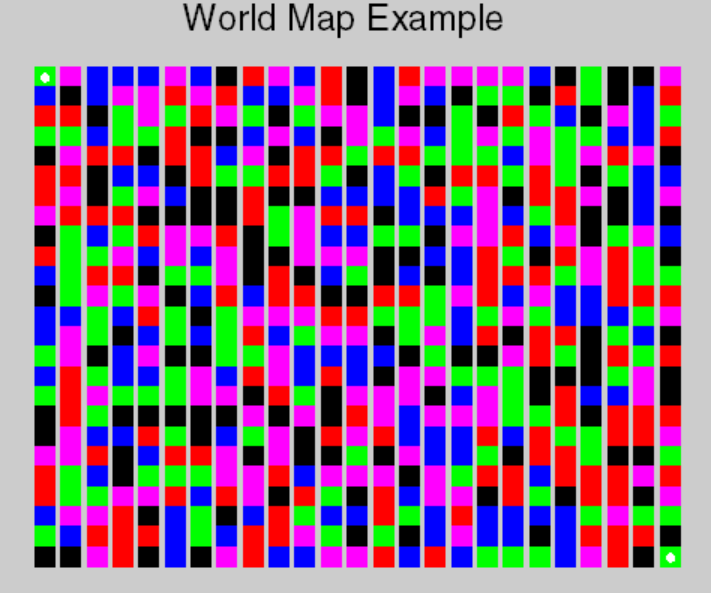
\includegraphics[scale=.5]{images/map-example.PNG}
\caption{Map Example with Terrain (Sand = Magenta, Forest = Green, Pavement = Black, Water = Blue, Misc. Debris = Red, Start/Goal = White dots)}
\label{fig:map-example}
\end{figure}

The world map matrix were at first predefined to validate the two algorithms (defined path from start to goal) and to find appropriate parameter values for the algorithms (punishment weight, discount factor, goal reward, etc).  The maps were then randomized for further testing.  The simulated robot navigating the map from the start (top left corner) to the goal (bottom right corner) had no prior knowledge of the terrain of the state it was in.  It did know the map, however.  As each algorithm was run, the value at each state was updated using a reward for the action chosen as well as a punishment which was determined by the sensor readings for each state. On a normalized average the punishments for each terrain type was as follows: sand 1, forest 2, pavement 0, water 3, mountainous rock/debris 4. This is much like the penalties incurred in James Sutton's puddle world problem, however, in this case the robot does not know about the terrain in its world, only what it reads through its sensors~\cite{sutton1996generalization}. Varying punishments made one state more favorable than another in terms of proximity to the goal, safeness, and efficiency. A rewards matrix of M*NxM*N was created, where each row symbolized a state and each column symbolized an action (next state).  Each neighbor state in the actions column were given a value of 0, non-neighbors were given a value of -\begin{math}\infty\end{math}. The goal state and any state that was a neighbor to the goal received the highest reward value.  A Q-matrix was also created the same way as the reward matrix, however, the goal was set to 0 to be updated by the temporal difference learning algorithms. Both the reward and Q-matrix represented the true map of the world without terrain information~\cite{tutorial}. Other factors needing tuning were the goal reward, the discount factor, and the punishment weight.  These were found for both algorithms through the control testing on a predefined map. Also, each algorithm was run for 10,000 episodes with an epsilon of 0.2 meaning that 20\% of the episodes would have next state actions chosen at random under the \begin{math}\epsilon\end{math}-greedy selection policy. The updated Q-matrix is used to determine the best path based on the highest rewards for each action at a given state.

\paragraph{Q-Learning Algorithm}
To implement the Q-learning algorithm, the high-level steps outlined in Algorithm \ref{alg:q-learning} were used.  As shown by the algorithm, a random state is chosen from the generated Q-matrix used to hold the values to determine the best path.  Then an action is taken in the current state based on the \begin{math}\epsilon\end{math}-greedy selection policy.  Using this action, the next state transition is determined as well as the reward for taking the action.  These values then update the Q-matrix at the current state as described by (\ref{eq:Q-learning value function}). This is then repeated with the next state, until the current state is the goal. As shown in the algorithm, the Q-matrix at each state is updated based on a learning parameter, \begin{math}\alpha\end{math} which is set to 1 in this application to assure quick learning. This matrix also depends on a discount factor denoted by \begin{math}\gamma\end{math} which is set to 0.8 to give importance to future rewards~\cite{Eden}. This was repeated for 10,000 episodes where at the start of each episode a random starting state was chosen. 

\begin{algorithm}
\caption{Q-Learning Algorithm~\cite{Eden}}
\label{alg:q-learning}
\begin{algorithmic} 
\For{e $\in$ number of episodes}
\State Pick random state $s$
\While {$s$ is not the goal}
\State Choose action $a$ from $s$ using epsilon policy from Q
\State Take action $a$, observe reward $r$ and next state $s'$
\State Update Q-values as follows:
\State $Q(s,a) \leftarrow Q(s,a) + \alpha [r+ \gamma*max_{\alpha}(Q(s',a')) - Q(s,a)] $
\State $s \leftarrow s'$
\EndWhile
\EndFor
\end{algorithmic}
\end{algorithm}



\paragraph{Sarsa Algorithm}
To implement the Sarsa algorithm, the high-level steps outlined in Algorithm \ref{alg:sarsa} were used.  As shown by the algorithm a random state is chosen from the generated Q-matrix used to hold the values to determine the best path.  Then an action is taken in the current state based on the \begin{math}\epsilon\end{math}-greedy selection policy.  Then until the state present is not the goal, the action will be taken and the next state transition is determined as well as the reward for taking the action. Another action is chosen using the \begin{math}\epsilon\end{math}-greedy selection policy for the next state. The Q-matrix at the current state is then updated as described in (\ref{eq:Sarsa value function}). As shown in the algorithm, the Q-matrix at each state is updated based on a learning parameter, \begin{math}\alpha\end{math} which is set to 1 to assure quick learning. This matrix also depends on a discount factor denoted by \begin{math}\gamma\end{math} which is set to 0.3 to give importance to future rewards~\cite{Eden}. This was repeated for 10,000 episodes where at the start of each episode a random starting state was chosen.



\begin{algorithm}
\caption{Sarsa Algorithm~\cite{Eden}}
\label{alg:sarsa}
\begin{algorithmic} 
\For{e $\in$ number of episodes}
\State Pick random state $s$
\State Choose action $a$ from $s$ using epsilon policy from Q
\While {$s$ is not the goal}
\State Take action $a$, observe reward $r$ and next state $s'$
\State Choose action $a'$ from $s'$ using epsilon policy from Q
\State Update Q-values as follows:
\State $Q(s,a) \leftarrow Q(s,a) + \alpha [r+ \gamma*max_{\alpha}(Q(s',a')) - Q(s,a)] $
\State $s \leftarrow s'$
\State $a \leftarrow a'$
\EndWhile
\EndFor
\end{algorithmic}
\end{algorithm}


\subsubsection{Results}

To validate the effectiveness of the two algorithms, each was run with a 5x5, 10x10, 15x15, and 25x25 size world with randomly generated terrains.  Each was run in 10 different terrain maps at each world size.  The results from this can be found in Table \ref{tab:results}.  As shown, it is apparent that the Q-Learning algorithm performs best in terms of cost.  It chooses the shortest and safest path. Also, as the world size gets bigger, the Q-Learning algorithm takes advantage of the increase in space and terrain to lower its cost per move. Sarsa also does this, but only slightly.  The Sarsa algorithm is the fastest, while it may not be the most efficient.  It is shown to finish well before the Q-Learning algorithm on larger maps.  However, the Q-Learning algorithm has a higher rate of convergence, where the Sarsa algorithm is prone to diverge at larger map sizes.  In the 25x25 world size, the Sarsa algorithm failed to converge, increasing the discount factor for the algorithm at this world size to 0.8 allowed for convergence. Examples of paths found by the Q-Learning algorithm and Sarsa algorithm at a world size of 25x25 are shown in Fig. \ref{fig:q-learning example} and Fig. \ref{fig:sarsa_example}, respectively.

In consideration of natural disaster relief and rebuilding, the Q-Learning algorithm is the best.  It takes the longest to converge, but will find the most efficient path, that is time conscience and safe for itself.  Sarsa, tends to favor the goal over safety in these situations because of its exploitation over exploration strategy. 


\begin{figure}
\centering
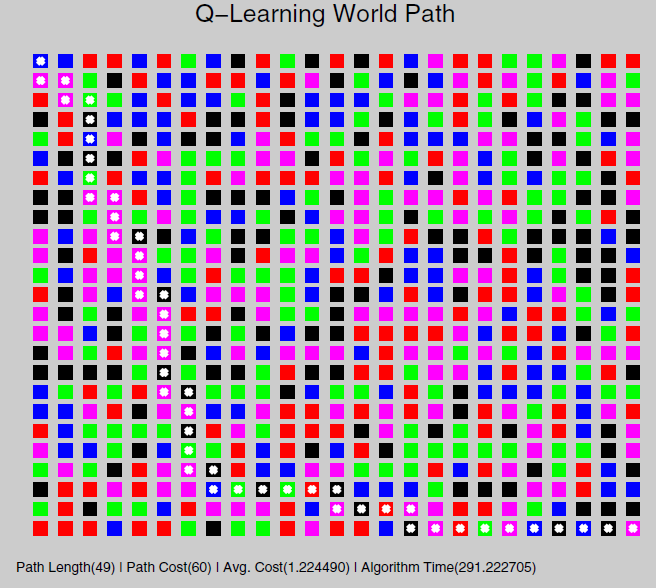
\includegraphics[scale=.75]{images/q-learning-example.PNG}
\caption{Q-Learning Algorithm Path Example with Punishment}
\label{fig:q-learning example}
\end{figure}

\begin{figure}
\centering
%\captionsetup{justification=centering}
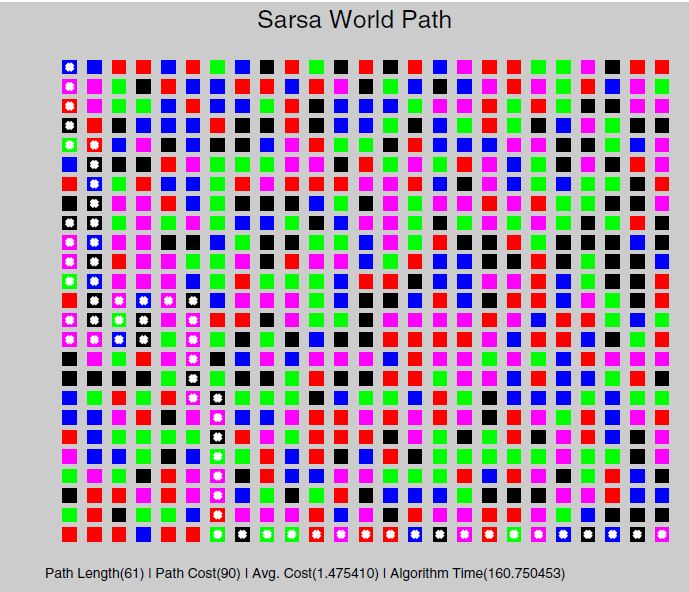
\includegraphics[scale=.75]{images/sarsa-example.PNG}
\caption{Sarsa Algorithm Path Example with Punishment}
\label{fig:sarsa_example}
\end{figure}

\begin{table}[]
\centering
%\captionsetup{justification=centering}
\caption{Q-Learning and Sarsa results across several world map sizes}
\label{tab:results}
\begin{tabular}{@{}llll@{}}
\toprule
\rowcolor[HTML]{FFFFFF} 
{\color[HTML]{333333} } & {\color[HTML]{333333} } & {\color[HTML]{333333} \textbf{Q-Learning}} & {\color[HTML]{333333} \textbf{Sarsa}} \\ \midrule
\rowcolor[HTML]{FFFFFF} 
\multicolumn{1}{|l|}{\cellcolor[HTML]{FFFFFF}{\color[HTML]{333333} }} & {\color[HTML]{333333} Avg. Path} & {\color[HTML]{333333} 9} & \multicolumn{1}{l|}{\cellcolor[HTML]{FFFFFF}{\color[HTML]{333333} 9}} \\
\rowcolor[HTML]{FFFFFF} 
\multicolumn{1}{|l|}{\cellcolor[HTML]{FFFFFF}{\color[HTML]{333333} }} & {\color[HTML]{333333} Avg. Cost} & {\color[HTML]{333333} 12.3} & \multicolumn{1}{l|}{\cellcolor[HTML]{FFFFFF}{\color[HTML]{333333} 18}} \\
\rowcolor[HTML]{FFFFFF} 
\multicolumn{1}{|l|}{\cellcolor[HTML]{FFFFFF}{\color[HTML]{333333} 5x5}} & {\color[HTML]{333333} Avg. Unit Cost} & {\color[HTML]{333333} 1.3667} & \multicolumn{1}{l|}{\cellcolor[HTML]{FFFFFF}{\color[HTML]{333333} 2.000}} \\
\rowcolor[HTML]{FFFFFF} 
\multicolumn{1}{|l|}{\cellcolor[HTML]{FFFFFF}{\color[HTML]{333333} }} & {\color[HTML]{333333} Avg. Time (s)} & {\color[HTML]{333333} 2.396} & \multicolumn{1}{l|}{\cellcolor[HTML]{FFFFFF}{\color[HTML]{333333} 2.2731}} \\
\rowcolor[HTML]{FFFFFF} 
\multicolumn{1}{|l|}{\cellcolor[HTML]{FFFFFF}{\color[HTML]{333333} }} & {\color[HTML]{333333} \% Converge} & {\color[HTML]{333333} 100} & \multicolumn{1}{l|}{\cellcolor[HTML]{FFFFFF}{\color[HTML]{333333} 100}} \\ \midrule
\rowcolor[HTML]{FFFFFF} 
\multicolumn{1}{|l|}{\cellcolor[HTML]{FFFFFF}{\color[HTML]{333333} }} & {\color[HTML]{333333} Avg. Path} & {\color[HTML]{333333} 19} & \multicolumn{1}{l|}{\cellcolor[HTML]{FFFFFF}{\color[HTML]{333333} 23.667}} \\
\rowcolor[HTML]{FFFFFF} 
\multicolumn{1}{|l|}{\cellcolor[HTML]{FFFFFF}{\color[HTML]{333333} }} & {\color[HTML]{333333} Avg. Cost} & {\color[HTML]{333333} 23.4} & \multicolumn{1}{l|}{\cellcolor[HTML]{FFFFFF}{\color[HTML]{333333} 38.8}} \\
\rowcolor[HTML]{FFFFFF} 
\multicolumn{1}{|l|}{\cellcolor[HTML]{FFFFFF}{\color[HTML]{333333} 10x10}} & {\color[HTML]{333333} Avg. Unit Cost} & {\color[HTML]{333333} 1.2316} & \multicolumn{1}{l|}{\cellcolor[HTML]{FFFFFF}{\color[HTML]{333333} 1.6260}} \\
\rowcolor[HTML]{FFFFFF} 
\multicolumn{1}{|l|}{\cellcolor[HTML]{FFFFFF}{\color[HTML]{333333} }} & {\color[HTML]{333333} Avg. Time (s)} & {\color[HTML]{333333} 12.7255} & \multicolumn{1}{l|}{\cellcolor[HTML]{FFFFFF}{\color[HTML]{333333} 12.2337}} \\
\rowcolor[HTML]{FFFFFF} 
\multicolumn{1}{|l|}{\cellcolor[HTML]{FFFFFF}{\color[HTML]{333333} }} & {\color[HTML]{333333} \% Converge} & {\color[HTML]{333333} 100} & \multicolumn{1}{l|}{\cellcolor[HTML]{FFFFFF}{\color[HTML]{333333} 60}} \\ \midrule
\rowcolor[HTML]{FFFFFF} 
\multicolumn{1}{|l|}{\cellcolor[HTML]{FFFFFF}{\color[HTML]{333333} }} & {\color[HTML]{333333} Avg. Path} & {\color[HTML]{333333} 29} & \multicolumn{1}{l|}{\cellcolor[HTML]{FFFFFF}{\color[HTML]{333333} 60.75}} \\
\rowcolor[HTML]{FFFFFF} 
\multicolumn{1}{|l|}{\cellcolor[HTML]{FFFFFF}{\color[HTML]{333333} }} & {\color[HTML]{333333} Avg. Cost} & {\color[HTML]{333333} 32.2} & \multicolumn{1}{l|}{\cellcolor[HTML]{FFFFFF}{\color[HTML]{333333} 80.0}} \\
\rowcolor[HTML]{FFFFFF} 
\multicolumn{1}{|l|}{\cellcolor[HTML]{FFFFFF}{\color[HTML]{333333} 15x15}} & {\color[HTML]{333333} Avg. Unit Cost} & {\color[HTML]{333333} 1.1103} & \multicolumn{1}{l|}{\cellcolor[HTML]{FFFFFF}{\color[HTML]{333333} 1.3110}} \\
\rowcolor[HTML]{FFFFFF} 
\multicolumn{1}{|l|}{\cellcolor[HTML]{FFFFFF}{\color[HTML]{333333} }} & {\color[HTML]{333333} Avg. Time (s)} & {\color[HTML]{333333} 37.8544} & \multicolumn{1}{l|}{\cellcolor[HTML]{FFFFFF}{\color[HTML]{333333} 33.4482}} \\
\rowcolor[HTML]{FFFFFF} 
\multicolumn{1}{|l|}{\cellcolor[HTML]{FFFFFF}{\color[HTML]{333333} }} & {\color[HTML]{333333} \% Converge} & {\color[HTML]{333333} 100} & \multicolumn{1}{l|}{\cellcolor[HTML]{FFFFFF}{\color[HTML]{333333} 40}} \\ \midrule
\rowcolor[HTML]{FFFFFF} 
\multicolumn{1}{|l|}{\cellcolor[HTML]{FFFFFF}{\color[HTML]{333333} }} & {\color[HTML]{333333} Avg. Path} & {\color[HTML]{333333} 49} & \multicolumn{1}{l|}{\cellcolor[HTML]{FFFFFF}{\color[HTML]{333333} 63.2*}} \\
\rowcolor[HTML]{FFFFFF} 
\multicolumn{1}{|l|}{\cellcolor[HTML]{FFFFFF}{\color[HTML]{333333} }} & {\color[HTML]{333333} Avg. Cost} & {\color[HTML]{333333} 51.3} & \multicolumn{1}{l|}{\cellcolor[HTML]{FFFFFF}{\color[HTML]{333333} 101*}} \\
\rowcolor[HTML]{FFFFFF} 
\multicolumn{1}{|l|}{\cellcolor[HTML]{FFFFFF}{\color[HTML]{333333} 25x25}} & {\color[HTML]{333333} Avg. Unit Cost} & {\color[HTML]{333333} 1.0469} & \multicolumn{1}{l|}{\cellcolor[HTML]{FFFFFF}{\color[HTML]{333333} 1.6005*}} \\
\rowcolor[HTML]{FFFFFF} 
\multicolumn{1}{|l|}{\cellcolor[HTML]{FFFFFF}{\color[HTML]{333333} }} & {\color[HTML]{333333} Avg. Time (s)} & {\color[HTML]{333333} 337.8118} & \multicolumn{1}{l|}{\cellcolor[HTML]{FFFFFF}{\color[HTML]{333333} 186.467*}} \\
\rowcolor[HTML]{FFFFFF} 
\multicolumn{1}{|l|}{\cellcolor[HTML]{FFFFFF}{\color[HTML]{333333} }} & {\color[HTML]{333333} \% Converge} & {\color[HTML]{333333} 100} & \multicolumn{1}{l|}{\cellcolor[HTML]{FFFFFF}{\color[HTML]{333333} 50*}} \\
\multicolumn{1}{|l|}{} & \multicolumn{3}{l|}{*with a discount factor of 0.8} \\ \bottomrule
\end{tabular}
\end{table}


\subsubsection{Conclusion}

Reinforcement learning is a series of methods and algorithms used to pseudo map out the way a living being makes decisions. Just like a living being, a decision cannot be proven right or wrong until it has been made~\cite{tutorial}. This methodology gives way for a system to learn its environment and discover patterns not easily recognizable. Used in the case of natural disaster response or ruins exploration, reinforcement learning, specifically temporal difference learning, can be used to explore the area, as well as build an efficient navigation map. In terms of the experiments done in this paper Q-Learning does much better than Sarsa in creating an efficient and safe path from a start to a goal.  Using multiple synchronized systems across a map, where each system would represent an episode, could reduce the time limitation found in Q-learning.  In this type of problem, Q-Learning does the best because of the importance it places on exploration.  On known, non-variable maps, Sarsa will do better because it can exploit rewards in future states early.




\section{Apprenticeship Learning (Inverse Reinforcement Learning)}
	Apprenticeship Learning, or inverse reinforcement learning, is the process of learning a cost/reward function to move from state to state. In these cases, the system observes and attempts to learn from another system that performs some task. Unlike reinforcement learning, the cost-function does not need to be known. Therefore, this type of system takes in an expert's policy (through demonstration) and learns a cost function based on its own state features and features perceived from the expert~\cite{jangir_2016}.		
		
		In \cite{hamahata2008effective} an imitation learning (inverse reinforcement learning) algorithm is used in two ways, one with supervised learning and one with reward shaping. In supervised learning, the imitator observes a demonstrator's motion and attempts to model it. One issue with this is that this is a black box learning technique.  The imitator can observe the final state of the demonstrator, but it has no knowledge of hidden states and actions used to create the motion. This can be mitigated if the imitator knows the inverse model of the demonstrator system. Hamahata et al. \cite{hamahata2008effective}, assumes that the imitator obtains the estimated actions over a discrete time from the demonstrator.  This then allows the imitator to find the optimal control to imitate the demonstrator using least squares or ridge regression. In reward shaping a more implicit approach to imitation learning is used. This method attempts to create a reward function from the observations of the demonstrator.  In many cases, changing a rewards function also changes the optimal policy of the system.  However, the rewards function found is designed to be included as an aggregate term to the underlying rewards function. The additional rewards function is defined as (~\ref{eq:additional_rewards}).
		\begin{equation}
            \label{eq:additional_rewards}
            \resizebox{0.44\textwidth}{!}{$r\textsuperscript{sub}\textsubscript{t+1}= \gamma\phi(x_{t+1})-\phi(x_{t})$}~\cite{hamahata2008effective}
        \end{equation}
		The value of this is added to the value of the underlying rewards function. In the additional rewards function, the \textit{$\phi$} term is defined when it is equal to the optimal value function. Using this shaping method the imitator has a faster learning rate~\cite{hamahata2008effective}.
		
		One challenge of inverse reinforcement learning is limited demonstrations and not performing the exact task as the demonstrator. In these cases, traditional imitation learning is not a feasible option. In \cite{atkeson1997robot} a method is proposed to learn an optimal policy rather than just a reward. This means that the system learns at the task level rather than just matching patterns which is useful for cases where the exact motion of the demonstrator is not learned. This paper explores the inverse pendulum problem, and attempts to solve it using reinforcement learning. This approach proved to be limited by intricately complex movements, however it did demonstrate a sense of learned movement from demonstration~\cite{atkeson1997robot}.

\subsection{Bayesian Inverse Reinforcement Learning}
One method of solving an inverse reinforcement learning problem is using a Bayesian process. Ramachandran et al. created a Bayesian Inverse Reinforcement Learning (BIRL) algorithm that allowed for imperfect and incomplete expert data~\cite{ramachandran2007bayesian}.  By using a probability distribution the uncertainty present in expert data sets can be modeled. This allows for complicated tasks to be learned since the transitions from state to state are not only stochastic but may be due to a complex reward function. To do this, a posterior distribution is derived for the rewards obtained from a prior distribution and a probabilistic model of the expert's actions given by the reward function.  Given a set of observations, \textit{O}, from an expert, \textit{X} two observations can be made: the expert is attempting to maximize its total accumulated reward, \textit{R}, and the expert executes on a fixed policy that does not change over time or based on a decision. Therefore, the Bayesian probability of \textit{k} observations given the reward can be assumed independent as shown in (\ref{eq:bayesianindep}).

\begin{equation}
            \label{eq:bayesianindep}
            \resizebox{0.60\textwidth}{!}{$Pr_X(O_X|R) = Pr_X(O_1|R)Pr_X(O_2|R)...Pr_X(O_k|R)$}~\cite{ramachandran2007bayesian}%
        \end{equation}
In terms of the expert, the goal is to maximize the accumulated reward which is equivalent to performing the action which causes a states \textit{$Q^*$} value to be maximum. Using this, the more confident we are in the expert's ability to choose a good action (denoted as $\alpha_X$) the likelihood increases on the prediction that the expert would choose action \textit{a} in state \textit{s}.  This is shown in (\ref{eq:bayseianliklihood}).

\begin{equation}
            \label{eq:bayseianliklihood}
            \resizebox{0.60\textwidth}{!}{$Pr_X(O_X|R) =  \frac{1}{Z}e^{\alpha_X\sum_{i}^{}Q^*(s_i,a_i,R)}$}~\cite{ramachandran2007bayesian}%
        \end{equation}
Where, $\sum_{i}^{}Q^*(s_i,a_i,R)$ is the expected value of the observations $(s_i,a_i)$ using $R$. $Z$ is a normalizing constant. To compute the posterior probability of the reward function Bayes theorem is used as shown in (\ref{eq:bayestheorem}).
\begin{equation}
            \label{eq:bayestheorem}
            \resizebox{0.60\textwidth}{!}{$Pr_X(R|O_X) =  \frac{Pr_X(O_X|R)Pr(R)}{Pr(O_X)}= \frac{1}{Z'}e^{\alpha_X\sum_{i}^{}Q^*(s_i,a_i,R)}*Pr(R)$}~\cite{ramachandran2007bayesian}%
        \end{equation}
To use this in Apprenticeship Learning tasks a policy loss function must be defined. The loss function (\ref{eq:bayesianloss}) for learning a policy $\pi$ is based on some norm ($p$) of the difference between the optimal values for each state achieved using the optimal policy for $R$ ($V^*(R)$) and the values for each state achieved using the learned policy for $R$ $\pi$ ($V^\pi(R)$).  The goal is to find the $\pi$ that will minimize the expected policy loss over the posterior distribution of R.  
\begin{equation}
            \label{eq:bayesianloss}
            \resizebox{0.60\textwidth}{!}{$L_{policy}^{p}(R|\pi)=\norm{V^*(R)-V^\pi(R)}_p$}~\cite{ramachandran2007bayesian}%
        \end{equation}
One challenge lies in the computation of a posterior distribution for $R$ at a specific point.  This is because this calculation relies on calculating the optimal Q-function which is not efficient.  Therefore a modification is made to release this constraint.  As the algorithm learns it keeps track of the policy ($\pi$) that is optimal for the current infered reward ($R$).  Using a uniform sampling ($\tilde{R}$) from the neigbors of $R$ the Q-values for $\pi$ are computed for all state-action pairs $(s,a)$, $Q^\pi(s,a,\tilde{R})$. If the Q-value for a state using $\pi$, ($Q^\pi(s,\pi(s),\tilde{R})$), is less than the Q-value for a state with any action, ($Q^\pi(s,a,\tilde{R})$), then, a new $\tilde{\pi}$ is found by updating the Q-values using policy iteration using expert data, $\tilde{R}$, and $\pi$. Then with probability of $\frac{f(\tilde{R},\tilde{\pi})}{f(R,\pi)}$ $R$ is set to $\tilde{R}$ and $\pi$ is set to $\tilde{\pi}$, otherwise only $R$ is set to $\tilde{R}$  with probability $\frac{f(\tilde{R},\tilde{\pi})}{f(R,\pi)}$.  This algorithm returns the final calculated $R$ after all iterations are complete~\cite{ramachandran2007bayesian}.

\subsection{Gaussian Process Inverse Reinforcement Learning}
\label{sec:gpirl}
An issue with many inverse reinforcement learning algorithms is that it assumes a linear reward function.  This limits the extent of what inverse reinforcement learning can learn from an expert.  For example, in a highway driving model used in~\cite{levine2011nonlinear} an agent needs to learn how to avoid cars going a fixed speed, choose the speed it is going, and make sure it is not speeding when it is within two car-lengths from a police vehicle.  The connection between the speed and proximity to a police vehicle makes the underlying reward function nonlinear. To learn nonlinear rewards Gaussian processes are used with inverse reinforcement learning, which is referred to as GPIRL~\cite{qiao2011inverse}~\cite{levine2011nonlinear}. A key to GPIRL's success is its ability to combine the probabistic reasoning of stochastic expert behavior with the ability to learn a nonlinear function of features for the reward~\cite{levine2011nonlinear}. As the name suggests, GPIRL is modeled as a Gaussian process whose structure is determined by a kernel function. In Gaussian process regression, the noisy observations $y$ of the true outputs $u$ are used.  GPIRL learns $u$ which in turn represents the rewards that are associated with the feature coordinates $X_u$. These coordinates can be the feature values of all states present or a subset of all states. Any state not present in the observations have their reward inferred by Gaussian process.  The goal of GPIRL is to learn the kernel hyper-parameters $\theta$ that reveals the structure of the reward ($r$). Therefore, the values of $u$ and $\theta$ are found by maximizing their probability with respect to the expert demonstrations $D$ as shown in (\ref{eq:GP_full}).

\begin{equation}
            \label{eq:GP_full}
            \resizebox{0.6\textwidth}{!}{$P(u,\theta|D,X_u)\propto P(D,u,\theta|X_u) = [\int_{r}P(D|r)P(r|u,\theta,X_u)dr]P(u,\theta|X_u) $}~\cite{levine2011nonlinear}%
        \end{equation}
Where $P(D|r)$ is the IRL term, $P(r|u,\theta,X_u)$ is the Gaussian process posterior, and $P(u,\theta|X_u)$ is the Gaussian process probability.  The Gaussian posterior represents the probability of the reward function with respect to $u$ and $\theta$. The Gaussian process probability is the prior probability of an assignment to $u$ and $\theta$. The log of this function gives the Gaussian process log marginal likelihood which will favor simple kernel functions and those values of $u$ that support the current kernel matrix.  Using the automatic relevance detection (ARD) kernel with $\theta = \{ \beta,\Lambda \}$ states with different highly-weighted features will take on different reward values whereas states with similar highly-weighted features will take on similar reward values. In this case $\beta$ is the overall variance and $\Lambda$ represents the weights on each feature. The process of learning $\Lambda$ gives features that are less relevant low weights and features that are very relevant high weights. One advantage to GPIRL is that while $X_u$ needs to cover the space of feature values, fewer points are needed than are states.  This is advantageous with problems with large state-spaces. In~\cite{levine2011nonlinear} $X_u$ contained feature values for all states visited in $D$, as well as additional random states to add to the overall count of $X_u$. 

Levine et al.~\cite{levine2011nonlinear} compared GPIRL performance to FIRL, MaxEnt, and MaxEnt/Lp. In the object world experiments it was shown that GPIRL needed significantly less expert demonstrations to converge to a solution when compared to the other algorithms. It was also shown that when novel states were presented GPIRL learned more accurate rewards than the other algorithms.  Using the highway driving model, an experiment with nonlinear rewards that was tough on many IRL algorithms, GPIRL was able to successfully learn the reward structure~\cite{levine2011nonlinear}. Qiao et al.~\cite{qiao2011inverse} also saw similar success with GPIRL.  In experiments they compared GPIRL with LIRL (linear inverse reinforcement learning) and CPIRL (convex programming inverse reinforcement learning). In the GridWorld experiment, each algorithm converged, however, GPIRL converged much faster than LIRL (2 times slower) and CPIRL (1.8 times slower).  They also used a discrete version of the hill climb problem where  environment information was skipped (partially observable).  GPIRL was able to successfully build the reward structure despite not having all of the information. Therefore, GPIRL was shown to be able to find the reward structure with fewer observations that were needed with LIRL and CPIRL~\cite{qiao2011inverse}.


\subsection{Maximum Entropy Inverse Reinforcement Learning}
\label{sec:maxentirl}
In many imitation learning problems modeling sequential decision-making behavior is often very difficult due to the lack of foresight in these systems. Ziebart et al.~\cite{ziebart2008maximum} developed an inverse reinforcement technique based on the principle of maximum entropy theory to counter this.  They tackled modeling real-world navigation and driving behaviors by sampling noisy and imperfect data from driving "experts".  Their approach was able to model route preferences of drivers as well as infer destinations and routes based on partial trajectories using GPS data of taxi-cab driving.  The environment they tested in was a known-fixed structure of the world (such as a road network) with known actions characterized by various road features such as speed limit and number of lanes.

The idea of inverse reinforcement learning revolves on an agent optimizing a function that linearly maps features of each state (\textit{$s_j$} to a reward value. Therefore, the reward value of an "expert" data sample, or trajectory, is a sum of state rewards which can be simplified to the reward weights, (\textit{$\theta$}), applied to the feature counts in a trajectory/path ($\zeta$) (\ref{eq:feature_counts}) as shown in (\ref{eq:feature_count_reward}).

\begin{equation}
            \label{eq:feature_counts}
            \resizebox{0.20\textwidth}{!}{$f\textsubscript{$\zeta$}= \sum_{s_j\in\zeta}^{}f\textsubscript{$s_j$}$}~\cite{ziebart2008maximum}%
        \end{equation}

\begin{equation}
            \label{eq:feature_count_reward}
            \resizebox{0.44\textwidth}{!}{$reward(f\textsubscript{$\zeta$})= \theta \cdot f\textsubscript{$\zeta$} = \sum_{s_j\in\zeta}^{}\theta \cdot f\textsubscript{$s_j$}$}~\cite{ziebart2008maximum}
        \end{equation}

A major problem of using "expert" trajectories is that an inverse reinforcement algorithm may find a preference for one path over others.  This poses a problem that an agent will only learn a path and not how features of a state can help in path decision making.  Using maximum entropy this problem is solved by choosing a distribution that does not exhibit preference beyond feature expectations.  Using this probabalistic model for deterministic (no randomness) path distributions, trajectories with the same final reward will be treated equally, where a preference will only be given for trajectories with higher reward.  Trajectories with a higher reward will have an exponentially higher probability. This is shown in (\ref{eq:maximum_entropy}), where \textit{Z($\theta$)} is the partition function which will always converge given trajectories that reach a reward-giving goal in a finite number of steps.

\begin{equation}
            \label{eq:maximum_entropy}
            \resizebox{0.44\textwidth}{!}{$reward(P(\zeta\textsubscript{i})|\theta)= \frac{1}{Z(\theta)} e^{\theta \cdot f_{\zeta_i}}=  \frac{1}{Z(\theta)} e^{\sum_{s_j\in\zeta_i}^{}\theta \cdot f\textsubscript{$s_j$}}$}~\cite{ziebart2008maximum}%
        \end{equation}

For non-deterministic (randomness) path distributions, (\ref{eq:maximum_entropy}) must be altered to take randomness in path distributions into account. Most MDPs (Marko Decision Process) that relate to real-world environments or dynamics will have non-deterministic transitions between states, meaning that an action that is supposed to transition to one state may not do so with some probability $\epsilon$.  Therefore, this distribution over paths produces a stochastic policy where the probability of an action is weighted by the expected rewards of all paths that begin with that action as shown in (\ref{eq:stochastic_policy}).

\begin{equation}
            \label{eq:stochastic_policy}
            \resizebox{0.44\textwidth}{!}{$reward(P(action | \theta, T) \propto \sum_{\zeta:action\in\zeta_{t=0}}^{}P(\zeta | \theta, T)$}~\cite{ziebart2008maximum}%
        \end{equation}

Therefore, to find the optimal weights the likelihood of the observed data is maximized under the maximum entropy distribution (\ref{eq:maxent_weight_update}). Since this function will be convex for deterministic MDPs the optima is found using the gradient  which is defined by the difference between the expected feature counts from the expert and the learner's expected feature counts represented in terms of expected state visitation frequencies, (${{}D_s}_{i}$).  The gradient descent for the weights is shown in (\ref{eq:maxent_gradient}). At the optima, the feature expectations will match which will state that the learner performs equivalently to the demonstrated behavior even if the reward weights found are not the same as the ground truth.

\begin{equation}
            \label{eq:maxent_weight_update}
            \resizebox{0.52\textwidth}{!}{$\theta^* = argmax_\theta L(\theta) = argmax_\theta * \sum_{trajectories}^{}\log(\tilde\zeta|\theta,T)$}~\cite{ziebart2008maximum}%
        \end{equation}

\begin{equation}
            \label{eq:maxent_gradient}
            \resizebox{0.44\textwidth}{!}{$\bigtriangledown L(\theta) = \tilde f - \sum_{\zeta}^{} P(\zeta|\theta,T)f_\zeta = \tilde f - \sum_{s_i}^{}D_{s_{i}}F_{s_{i}}$}~\cite{ziebart2008maximum}%
        \end{equation}

This paper~\cite{ziebart2008maximum} uses Maximum Entropy IRL to recover a reward function for predicting driving behavior and route recommendation. The model of this problem contained over 300,000 states (road segments) and 900,000 actions. All expert trajectories were assumed to reach a goal while optimizing time, safety, stress, fuel costs, and maintenance costs. This is used as the cost function for this system, whereas the destination for all trajectories is the state where no additional cost is incurred. The expert trajectories were GPS traces from 25 taxi drivers which resulted in over 100,000 miles of collected data over 3,000 hours of driving. Each state (road segment) was characterized by: road type, speed, lanes, and transitions. Using the Maximum Entropy IRL model this paper achieved state-of-the-art results for its time for path matching.


\subsection{IRL using DQN}
One modification to inverse reinforcement is using a DQN (such as the one in section~\ref{sec:dqn}) in the value iteration step to determine the Q-values. Sharifzadeh et al.~\cite{sharifzadeh2016learning} used this type of network to teach a simulation to drive in a highway environment. The agent was placed in a 3 lane highway and expert data was used to teach it to merge into lanes and not hit cars using three actions (forward, right, left).  The inputs to the system were values of 13 sensors that were discretized into 16 bins of visibility that indicated whether or not their was an obstacle. This resulted in 208 binary features which allowed for $2^{52}$ states. These the feature weights obtained from the IRL step were fed into the DQN to produce an output value for each action, or policy. The DQN step is shown in Fig.~\ref{fig:irl-dqn}.
\begin{figure}
\centering
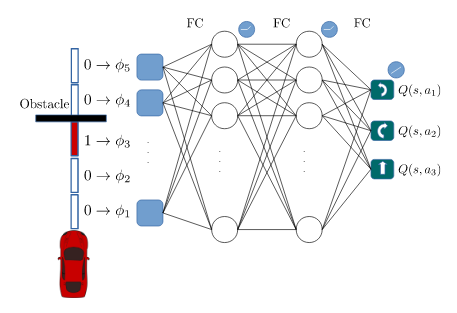
\includegraphics[scale=1]{images/irl-dqn.png}
\caption{Deep Q-Network Architecture in IRL~\cite{sharifzadeh2016learning}}
\label{fig:irl-dqn}
\end{figure}
Through experimentation it was shown that the reward was successfully able to be extracted from expert demonstrations in large state spaces.


\section{Deep Reinforcement Learning}
An advantage to using neural networks with inverse reinforcement learning stems from that fact that not everything can be observed. The demonstrator, or "expert", may not reach every state or may move in a stochastic fashion. Therefore, neural networks allow the system to generalize for unknown states and obstacles. Also, for complex systems with numerous state-action pairs, maintaining a Q-table with that much data becomes infeasible. Neural Networks are great for finding complex features in complex functions, therefore, the traditional \textit{Q-function} is replaced by a network~\cite{matiisen_2015}. The Neural Inverse Reinforcement Learning algorithm in~\cite{xia2016neural} is a model-free implementation of deep reinforcement learning. It uses several sensors on the robot as inputs into the neural network.  It also uses the current state, and any obstacle detected as inputs. Therefore, this method separates a robot's coordinates with its environment so that it can better generalize its navigation~\cite{xia2016neural}. Beyond just using neural networks for advanced reinforcement learning techniques, deep networks have become common practice. Deep networks allow agents to learn environments without the need to handcraft features or to have full observability of the environment. Often these networks use image data and several network layers to learn complex tasks~\cite{atari}.
	
	Atari has been a common platform for Deep Reinforcement Learning. Specifically, Deep Q-networks (DQN) developed by DeepMind (owned by Google) uses pixels and scores from classic Atari games to learn the cost function for the games to maximize the score~\cite{mnih2015human}. Most neural network implementations of Q-learning are unstable or fail to converge due to non-linear functions. By using deep convolutional neural networks and storing an agent's experience in replay memory a more stable loss function can be determined.   This method also applies Q-learning updates on mini-batches of experience that are drawn at random from a pool of samples generated by the system's own exploration. Therefore, the system is generating its own dataset to learn from. While this has been a proven method to increase the efficiency of the system, especially when using a GPU, this also allows the system to not get stuck in a Markov loop which causes divergence because of high correlations between state spaces.  This idea was further built upon by the authors in a paper published one year later~\cite{mnih2016asynchronous}. In this paper, the algorithm was modified to use multiple agents to learn rather than batch-processing (replay). This method further uncorrelated state spaces because different agents would be at different states. This method proved to converge much faster, and also learn unknown environments better~\cite{mnih2016asynchronous}. However, having multiple agents in a non-simulated environment can prove to be a challenge, therefore batch-processing as introduced in~\cite{mnih2015human} is a more feasible option. Another implementation of this algorithm is Maximum Entropy Deep Inverse Reinforcement Learning from ~\cite{wulfmeier2015maximum}. This algorithm applies wide convolutional layers to learn more relevant spatial features in the data it is trying to learn from. These wider convolutional layers essentially represent fully convolutional neural networks with width one. This essentially means that there is no pooling using this methodology to ensure every bit of raw input is used. 
	
	Unfortunately, reinforcement techniques lacked a benchmark.  An algorithm could not be compared directly to another algorithm on performance unless the same exact task was being done.  However, a benchmark was created in~\cite{duan2016benchmarking} for continuous control reinforcement learning tasks based on control, humanoid locomotion, occluded tasks, sensor limits, delayed action, combinational tasks. To do this all tasks were standardized into a finite-Markov decision process. Therefore, these benchmarking standards will be used to compare against future advancements in Deep Reinforcement Learning. 

\subsection{Deep Q-Networks (DQN)}
\label{sec:dqn}
Mnih et al.~\cite{atari} pioneered the use of deep neural networks in reinforcement learning to learn a variety of Atari 2600 games.  This work has been highly cited, and has led as a base for further advancements in deep reinforcement learning~\cite{atari}.  They use the idea of Deep Q-Networks (DQN) which uses a deep neural network to approximate the Q-function (\ref{eq:Q-learning value function}). This network takes as an input raw image data from a game (state) and outputs an action. The score of the game at each given state is fed in as the reward function, and the weights are iteratively optimized to achieve the highest score. The game state image passes through several convolutional layers before going into a fully connected layer to determine the next action out of 18 possible actions, this is shown in Fig.~\ref{fig:DQN-atari}. However, do the unstable nature of reinforcement learning when using nonlinear function approximators (neural networks), this method has many faults. Correlations in sequences of observations may cause Q values to drastically change during training causing the algorithm to diverge. Two methods used to overcome this instability are experience replay and a separate target network. Using these methods, DQN was able to provide a general framework to learn many Atari 2600 games at human or super-human levels. Basic games such as Pinball, Pong, Space Invaders, and Brick Breaker performed at super human levels. More complicated games with multiple goals or sequence restricted navigation performed well below human level such as Ms. Pac-Man, Alien, and River Raid~\cite{atari}.

\begin{figure}
\centering
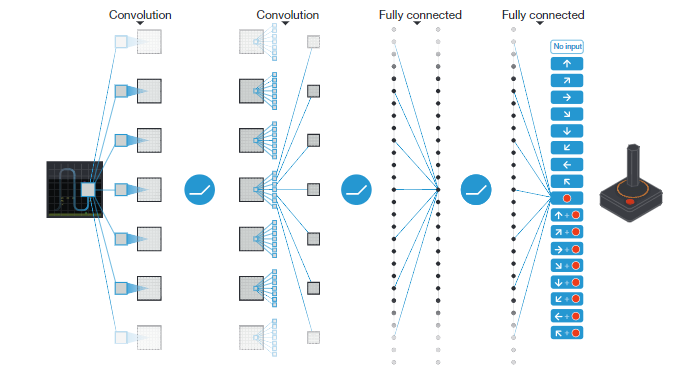
\includegraphics[scale=.95]{images/DQN-atari.png}
\caption{Deep Q-Network Architecture. The input consists of an 84x84x4 image. Each hidden layer is followed by a rectifier non-linearity (max(0,x)).~\cite{atari}}
\label{fig:DQN-atari}
\end{figure}


\subsubsection{Experience Replay}

Experience replay is inspired by nature in the idea that learning a task can be learned better if an agent (human or animal) uses their past learnings.  Therefore, as the network is being trained experience data from the agent is stored in state-action-reward-nextState pairs ($<s,a,r,s^{*}>$). Batches of these experiences are drawn at random during training from an experience replay buffer which contains a set number of experiences.  As a new experience is learned it is added to the buffer and the oldest replay is removed. These batch experiences are used to update the weights of the network as the network navigates through a sequence of observations.  This allows the network to learn from a variety of past experience instead of finding a local minima in the immediate episode it is learning in~\cite{atari}.

\subsubsection{Seperate Target Network}

One main issue with Q-learning based reinforcement learning is that Q values are constantly shifted by small amounts during every iteration.  These constant shifts in values can cause a network to easily diverge, especially early on when the updates have a larger magnitude.  Using a separate target network with Q values that is only updated periodically is one solution to this problem.  The network continues to update Q values iteratively, however, it will use the target network Q values in its calculations.  The target Q values are then updated periodically (adjustable hyper-parameter) with the current calculated Q values in the network.  This gives the system stability, and removes tightly coupled correlations from influencing the network weights~\cite{atari}.


\subsection{Double Deep Q-Networks (DDQN)}

One set back found from using the traditional DQN~\cite{atari} is that it may overestimate Q values for certain actions in a state~\cite{van2016deep}. This poses a problem if Q values for actions were not overestimated equally which is usually the case.  Therefore, during training there is a high chance that some sub-optimal actions may be given a high Q value early on which would cause the system to fall into a local minima.  Therefore Hasselt et al.~\cite{van2016deep} developed a technique called double DQN (DDQN) which utilized the network Q values and target-Q values.  In DQNs the max over Q values is used to compute the target-Q value, in double DQN the Q-values from the primary network are used to choose an action while the target-Q network is used to generate the target Q-value for the chosen action. Therefore, the action choice and target Q-value generation are decoupled which reduces overestimation and provides greater stability.  In~\cite{van2016deep}  the DDQN outperformed DQN on every Atari 2600 game except for two. The DDQN was also able to achieve super human level in games where DQN could not. 

\subsection{Dueling Deep Q-Networks (Dueling DQN)}
\label{sec:DuelingDQN}
With the idea that Q-values directly correspond to how beneficial it is to take action ($a$) in a given state. Traditionally, this is used in this context, however Wang et al.~\cite{wang2015dueling} splits these Q-values into two separate values.  One of the values is $V(s)$ which states how good it is to be in a given state. The second value is $A(a)$ which is the advantage function stating the advantage of taking action $a$ compared to the other possible actions.  Therefore, Q is decomposed as show in (\ref{eq:duelingQ})~\cite{wang2015dueling}.

\begin{equation}
          \label{eq:duelingQ}
          \resizebox{0.4\textwidth}{!}{$Q(s,a) = V(s) + A(a)$}~\cite{wang2015dueling}%
\end{equation}
Therefore, dueling DQNs contain two networks, one to compute $V(s)$ and one to compute $A(a)$.  The outputs of these networks are then combined to find the final Q-value ($Q(s,a)$) as shown in Fig.~\ref{fig:duelingDQN}~\cite{wang2015dueling}.

\begin{figure}
\centering
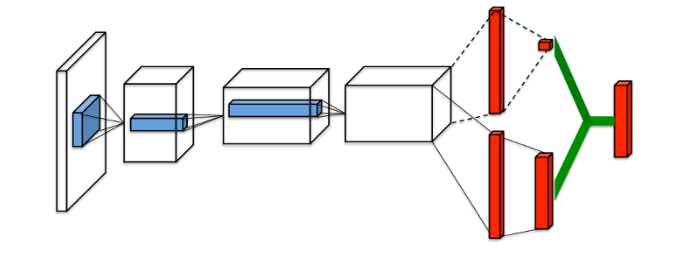
\includegraphics[scale=.85]{images/duelingDQN.png}
\caption{Dueling Deep Q-Network Architecture. Two networks are used and combined at the end.~\cite{wang2015dueling}}
\label{fig:duelingDQN}
\end{figure}

The idea of separating Q-values into these two value functions is to be able to create robust state value estimates without having it to be attached to a specific action.  For example, consider an agent in a room where it receives a very high reward of being in the green zone and a very low reward of being in the red zone. If the agent is in the green zone it is highly rewarding to be in that zone, and no action needs to be taken to receive reward. Therefore, it does not make sense in this case to consider the value of being in the green zone state being coupled with an action. Therefore, by decoupling the value of being in a state and the advantage of taking an action more complex and robust estimates can be made that allow for greater stability and faster learning~\cite{wang2015dueling}. This paper~\cite{wang2015dueling} also used Atari 2600 as its bench mark and greatly outperformed both DDQN and DQN architectures. 

\subsection{Deep Recurrent Q-Networks (DRQN)}
In DQNs~\cite{atari}, DDQNs~\cite{van2016deep}, and Dueling DQNs~\cite{wang2015dueling} allow the agent to have full access to the information of the environment. In other words, our system has full observability in that it is given full state information of the entire game state.  For example, grid worlds and Atari 2600 games have all the information of the world in a single state (no scrolling game play or worlds). However most real world problems will not give an agent full observability. Assume an agent does not have access to all the information in a world (partial observability), traditional DQN methods will not be able to converge. For example, in cases where there are walls or doors an agent will not know the states that are on the other side. Also, while spatial limitations exist, temporal information is also crucial.  Often, in single image inputs motion, speed, and direction can be lost to an agent. Even in DQN architectures, only 4 frames are used as an input, therefore in environments where past information is even more crucial these 4 frames greatly limit what can be learned. Environments where all information is not available to an agent are called Partially Observable Markov Decision Processes (POMDPs).  

Hausknecht et al.~\cite{HausknechtDRQN} found that the performance of DQNs decline when trying to learn a POMDP and could be better learned using recurrent neural networks. This created the Deep Recurrent Q-Network (DRQN) architecture. Instead of passing in a series of images as input to the network, DRQNs take in a single image. The difference lies in the first fully-connected layer being replaced with a recurrent LSTM layer. This change can be seen in Fig.~\ref{fig:drqn-arch}~\cite{HausknechtDRQN}.

\begin{figure}
\centering
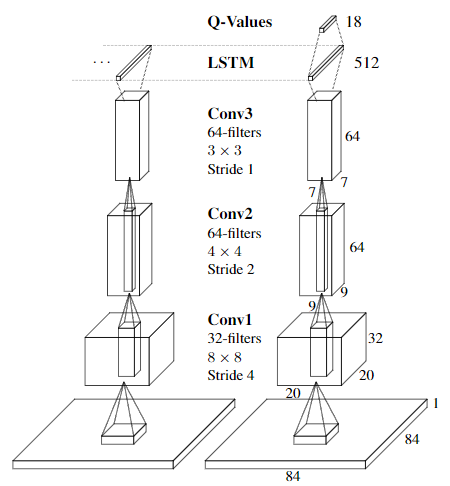
\includegraphics[scale=.85]{images/drqn-arch.png}
\caption{DRQN Architecture~\cite{HausknechtDRQN}.}
\label{fig:drqn-arch}
\end{figure}

As shown, the LSTM layer is inserted just before the value and advantage layers are calculated the same as in dueling DRQNs. Another change in this network is in the experience replay.  Instead of selecting a random batch of experiences, DRQNs train on random batches of sequence of experiences at a set length.  This is important so that sequences can be learned which is crucial to the recurrent nature of DRQNs. Using this network with the Atari 2600 framework, DRQNs showed significant improvement on POMDP style game play~\cite{HausknechtDRQN}. 

\section{Deep Inverse Reinforcement Learning}
A relatively new field that has come into the realm of reinforcement learning is Deep Inverse Reinforcement Learning (Deep IRL) or Deep Apprenticeship Learning.  This is the idea of using expert data to teach systems complex tasks.  Just as in reinforcement learning, the Deep IRL networks take in complex data types, such as images.  However, just as in regular IRL, these networks do not find a policy, but instead find a reward structure based on learning a policy from an expert.  There are many challenges to this, in that the reward function an expert uses is assumed to not be known.  The expert is assumed to make optimal and perfect moves, however, ideally many of these datasets come from experts behaving in a stochastic manner.  Expert data that is not stochastic brings about an issue of the expert not exploring its entire world, meaning when the system encounters a state that it did not learn from the expert it is unable to generalize well.  

Unlike in deep reinforcement learning, research using raw pixel images in this area is limited.  Much of the expert data is displayed as trajectory movements or direct observations from an expert.  While this works, it does not generalize well to tasks in the real world where only a series of videos may be available to learn from.  The issue with pixel data is that the system must first understand task it is seeing, extract the policy from the expert, then create a generalized reward system for an agent to follow.  This makes it a much more complex task than reinforcement learning, but its a task that is needed to be solved to expand deep learning to agents in the real world.

\subsection{Deep Gaussian Process IRL}
Jin et al.~\cite{jin2015inverse} took the successful GPIRL architecture from section \ref{sec:gpirl} and modified it to work in a deep network. This furthers the advantages of Gaussian process by allowing to learn even more complex reward structures across very large state spaces with limited expert demonstrations. Another advantage of using a deep network for GPIRL is that is not reliant on predefined features like its non-deep counterpart.  This allows for learning more complex reward structures from complex tasks where features may not be obvious.  Deep GPIRL uses a deep belief network with Gaussian process and Gaussian process latent variable model layers. Its goal is to learn an abstract reward structure using small data sets which mimics a human's ability to perform inductive reasoning after a few experiences. The Deep GPIRL architecture is shown in Fig.~\ref{fig:dgpirl-arch}.
\begin{figure}
\centering
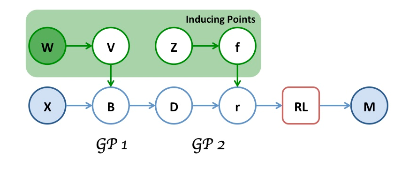
\includegraphics[scale=1]{images/dgpirl-arch.png}
\caption{Deep GPIRL Architecture~\cite{jin2015inverse}.}
\label{fig:dgpirl-arch}
\end{figure}
 As shown, $W$ stands for inducing points for the first Gaussian process layer which are small set of data points that are learned or selected directly. $V$ is the learned distribution, or selection, of those points.  $Z$ and $f$ act in a similar fashion for the second Gaussian process layer. $B$ and $D$ are the latent and noisy outputs from the first Gaussian process layer. $X$ is the state feature representation, $r$ is the learned latent reward that is learned from $X$ to explain the demonstrations $M$.  Using the Deep GPIRL in experiments, particularly ObjectWorld and BinaryWorld, it performs better than traditional IRL algorithms using fewer demonstrations. 

\label{sec:maxentdeepirl}
\subsection{Deep Maximum Entropy IRL}
Wulfmeier et al.~\cite{wulfmeier2015maximum} used multi-layer neural networks to implement Section~\ref{sec:maxentirl} without the need to hand-craft features. Using similar grid environments as~\cite{ziebart2008maximum}, a neural network (specifically a Fully Convolutional Neural Network) with wide convolutional layers (width one) is used to learn spatial features based on raw input.  

The first tests of this network used a regular neural network structure without any convolution layers, therefore the inputs were expert trajectories. The output of this neural network is used to estimate the reward function as is done in traditional inverse reinforcement algorithms. The input of this network is expert demonstrations ($\mu_{D}^{a}$) of state ($s$), action ($a$), reward pairing. The high level algorithm deals with iterating over \textit{n} epochs which represent the amount of gradient descent iterations. First, randomly intialized weights ($\alpha$) are forward propagated in the neural network.  The reward ($r^n$) is then extracted from this model and used to find an approximate policy ($\pi^n$) using value iteration. This policy is then used to find the expected state visitation frequency ($E|\mu^n|$) for each state (\textit{s}) as defined in Section~\ref{sec:maxentirl}.  The maximum entropy loss is found by (\ref{eq:maximum_entropy_loss}) using maximum entropy theory. The gradient is computed by taking the gradient of (\ref{eq:maximum_entropy_loss}) with respect to the reward ($r^n$) which is equivalent to the difference of the expected state visitation frequency of the expert ($\mu_D$) and learner expected state visitation frequency ($E|\mu^n|$) as shown in (\ref{eq:maximum_entropy_gradient}).  This is the same gradient calculation as found in~\cite{ziebart2008maximum}.  This gradient is then back-propagated through the network to update nodes.  The weights ($\alpha$) are then also updated with this gradient and the algorithm repeats until the number of epochs is reached. 

\begin{equation}
            \label{eq:maximum_entropy_loss}
            \resizebox{0.3\textwidth}{!}{$L_{D}^{n}=log(\pi^n) \times \mu_{D}^{a} $}~\cite{wulfmeier2015maximum}% 
        \end{equation}

\begin{equation}
            \label{eq:maximum_entropy_gradient}
            \resizebox{0.3\textwidth}{!}{$\frac{\delta L_{D}^{n}}{\delta r^{n}}=\mu_D -  E|\mu^n|$}~\cite{wulfmeier2015maximum}% 
        \end{equation}

This paper implemented and analyzed their DeepIRL solution on two types of environments, Objectworld and Binaryworld. An objectworld consists of an $M$x$M$ grid representing $M^2$ possible states.  There are 4 possible actions for an agent to move (up, down, left, right, stay in place). The state features are defined as the minimum distance to colored object.  The objects can be one of $C$ colors. The reward is defined as positive for grid cells which are distance 3 of color 1 and distance 2 of color 2. The reward is defined as negative for grid cells which are only within distance 3 of color 1, and zero otherwise.  The binary world consists of states being randomly assigned blue or red.  The feature vector for each state is a binary vector of length 9 which encoded the color of each cell in a 3x3 neighborhood. The reward is positive if 4 out of 9 neighboring states are blue, negative if exactly 5 are blue, and zero otherwise.  The binary world relies on a direct relationship between states which makes it a unique, and complex problem to solve. For both worlds the DeepIRL network produced state of the art results, however, inclusion of convolutional layers (Fully Convolutional Neural Network [FCNN] with width one) allows for the input of raw input without the need of hand-crafted features (such as what is needed for object world and binary world). The raw input is the entire state-space with what each state occupies (objects for object world, color for binary world). This allows the network to not only learn an appropriate reward function but also spatial features of the input environment in terms of the expert trajectory data.  One drawback of this is that more expert samples are needed for training to match performance of DeepIRL network without a CNN, however, this extends this architecture to take in raw image data to learn complex tasks in complex environments~\cite{wulfmeier2015maximum}.

\subsection{Deep Apprenticeship Learning (DAL)}
\label{sec:DAL}
Markovikj~\cite{markovikj2014deep} used a deep architecture to perform IRL on various games using raw pixel inputs. These games were Atari games; Freeway, Space Invaders, Seaquest. This was done through the creation of a multi-part architecture known as Deep Apprenticeship Learning. The two parts of this architecture are Deep Apprenticeship Q-Network (DAQN) and Deep Apprenticeship Reward Network (DARN).
\subsubsection{Deep Apprenticeship Q-Network (DAQN)}
The DAQN~\cite{markovikj2014deep} is used to take in raw inputs from expert game play ($D_E$) to learn a reward (or score) function which rates actions for states, much like the Q-function. Therefore, training this network will output the expert's policy. This network created using convolutional layers, similar to the Deep Q-Network~\cite{atari}. The inputs to this network are 83x83 raw pixel images.  Tests were done with feeding in 1-4 frames per input. The network was updated using batch processing of 32 samples. The structure is shown in Fig.~\ref{fig:daqn-dal}.
\begin{figure}
\centering
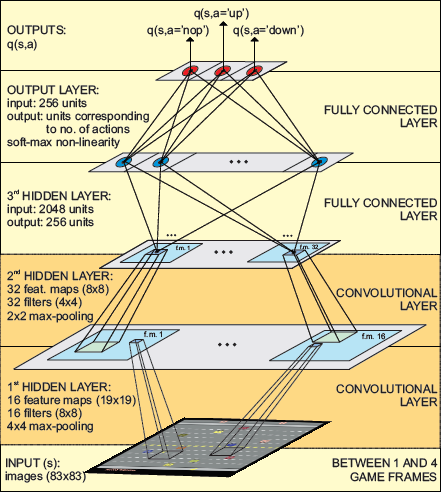
\includegraphics[scale=1]{images/daqn-dal.png}
\caption{DAQN Architecture~\cite{markovikj2014deep}.}
\label{fig:daqn-dal}
\end{figure}
As shown, this architecture outputs a softmax prediction between three possible actions (stay, up, down).  Therefore, for every state (raw pixel input) the network predicts the next action to be taken. The loss function of this network is shown in~\ref{eq:daqn-loss}.
\begin{equation}
     \label{eq:daqn-loss}
     \resizebox{0.5\textwidth}{!}{$J(w) =\sum_{a}[q_w(s,a)-\hat{q}(s,a)]^2$}~\cite{markovikj2014deep}% 
\end{equation}
Where, $w$ are the learned weights, $q_w(s,a)$ is the output of the DAQN and $\hat{q}(s,a)$ is the actual action taken by the expert represented by a 1-hot array.  Therefore, for inputs ($s=s_n,a=a_n \in D_E$), the array $\hat{q}$ is 1 if $a = a_n$ and 0 otherwise. The network is updated using AdaGrad where each parameter has its own learning rate, $\eta$ learned over time.

\subsubsection{Deep Apprenticeship Reward Network (DARN)}
Once the DAQN is trained, the DARN~\cite{markovikj2014deep} is used to extract the reward function from the learned expert policy in the DAQN.  The DARN has the same architecture as the DAQN (shown in Fig.~\ref{fig:daqn-dal}). However, it uses the output from the DAQN before the softmax in its loss function.  The input to DARN is a $(s,a,s')$ pairing where $s$ is an 83x83 image, $a$ is the action taken at that state, and $s'$ is the next state after taking action $a$ from state $s$. The loss function for DARN uses an L2-norm and is shown in~\ref{eq:darn-loss}.
\begin{equation}
     \label{eq:darn-loss}
     \resizebox{0.5\textwidth}{!}{$J_r(w) =\|r_w(s,a) - \hat{r}(s,a) \|_2$}~\cite{markovikj2014deep}% 
\end{equation}
Where, $w$ are the learned weights, $r_w(s,a)$ is the output of the DARN and $\hat{r}(s,a)$ is a Bellman representation of the DAQN~\ref{eq:darn-bellman}.
\begin{equation}
     \label{eq:darn-bellman}
     \resizebox{0.7\textwidth}{!}{$\hat{r}(s,a) = DAQN^{PRESOFT}(s,a) - \gamma \max_{a'}DAQN^{PRESOFT}(s',a')$}~\cite{markovikj2014deep}% 
\end{equation}
Where, $DAQN^{PRESOFT}(s,a)$ are the presoft values of the DAQN with inputs $(s,a)$ and $\max_{a'}DAQN^{PRESOFT}(s',a')$ is the maximum presoft value of the DAQN with inputs $(s',a')$. $\gamma$ is the discount factor on how much to weight future states. Therefore, the expanded loss function for the DAQN is shown in~\ref{eq:darn-loss-expanded}.  The overall training architecture for DARN is shown in Fig.~\ref{fig:darn-dal}.
\begin{equation}
     \label{eq:darn-loss-expanded}
     \resizebox{0.7\textwidth}{!}{$J_r(w) =\|r_w(s,a) - (DAQN^{PRESOFT}(s,a) - \gamma \max_{a'}DAQN^{PRESOFT}(s',a'))\|_2$}~\cite{markovikj2014deep}% 
\end{equation}
\begin{figure}
\centering
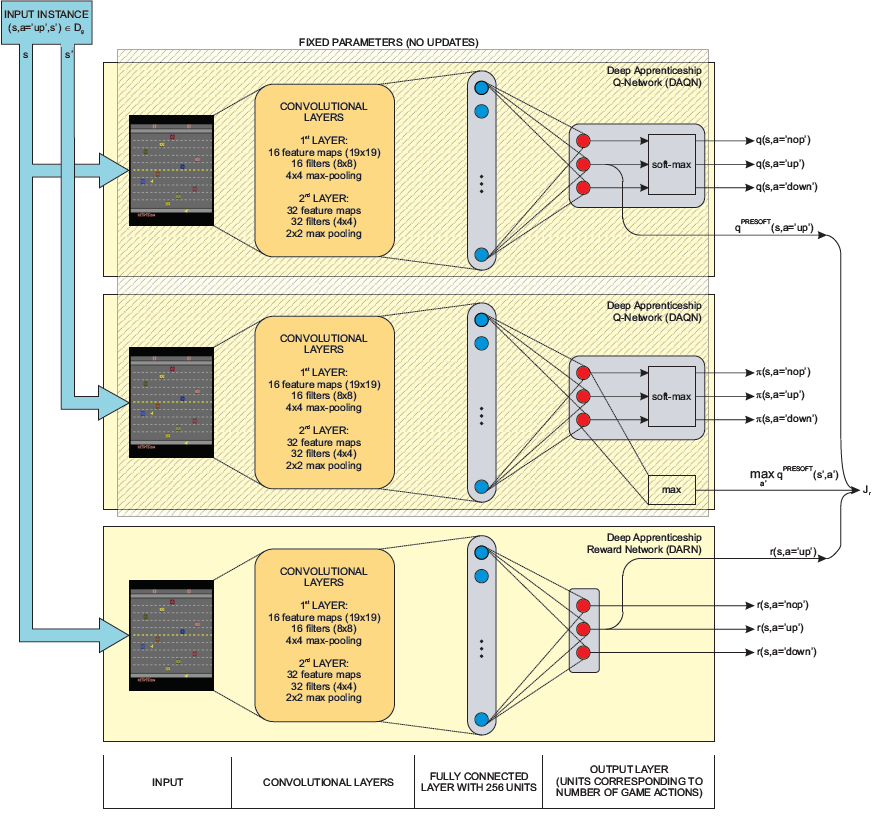
\includegraphics[scale=1]{images/darn-dal.png}
\caption{DAL Architecture~\cite{markovikj2014deep}.}
\label{fig:darn-dal}
\end{figure}
The DARN is trained using random state transitions contained in a separate dataset from the expert data, $D_g$.  This allows the system to generalize to all states, even ones not explored by the expert. 

\subsubsection{Results}
Once training on the DARN is complete, the system can now be used to predict next actions given a state. Due to the complexity of Space Invaders, this type of network did not generalize to its game play. However, it performed extremely well on the simple game of Freeway, obtaining a score much higher than other non-deep IRL algorithms~\cite{markovikj2014deep}. 

\subsection{Deep Q-Learning from Demonstrations (DQfD)}
Hester et al. undertook the challenge of bringing deep reinforcement learning to real world tasks~\cite{hester2017learning}.  They recognized, that while exploration in traditional reinforcement learning works well in simulation, it is not practical in physical environments.  Instead, they propose an algorithm that extends traditional DQNs to train with expert data using transfer learning theory.  They use important aspects of DQN such as Double DQN and experience replay.  To update the Q-values of the network with values from the target network the cost function in (\ref{eq:ddqn-dqfd}) is used.
\begin{equation}
     \label{eq:ddqn-dqfd}
     \resizebox{0.5\textwidth}{!}{$J_{DQ}(Q) =(R(s,a)+\gamma Q(s_{t+1},a^{max}_{t+1};\theta')-Q(s,a;\theta))^2$}~\cite{hester2017learning}% 
\end{equation}
Where $\theta'$ are the parameters of the target network, and $\theta$ are the parameters of the current network~\cite{van2016deep}.  However, due to the supervised learning step of using expert demonstrations, the cost function needs to be updated to include  (\ref{eq:ddqn-dqfd}).
\begin{equation}
     \label{eq:ddqn-dqfd}
     \resizebox{0.5\textwidth}{!}{$J_{E}(Q) =max_{a\in A}[Q(s,a)+l(s,a_E,a)]-Q(s,a_E)$}~\cite{hester2017learning}% 
\end{equation}
Where $a_E$ is the action the expert takes in state $s$.  $l(s,a_E,a)$ is a margin function where it is 0 when $a=a_E$ and a positive number (usually 1) otherwise.  This will allow for the expert's decisions to be weighted higher.  An L2 regularization term is also used and applied to the weights and biases of the network to prevent from over-fitting on small expert datasets.  Therefore, the entire loss function is (\ref{eq:ddqn-dqfd}).
\begin{equation}
     \label{eq:ddqn-dqfd}
     \resizebox{0.5\textwidth}{!}{$J(Q) =J_{DQ}(Q) + \lambda_1J_E(Q) + \lambda_2J_{L2}(Q)$}~\cite{hester2017learning}% 
\end{equation}
Where $\lambda_1$ and $\lambda_2$ are weights for each of the losses. For experience replay, with probability $p$ an expert experience $(s,a,s',reward)$ will be chosen from the entire set of expert demonstrations and with probability $1-p$ a random demonstration will be chosen from the set of agent's experience held in a limited buffer.  When the buffer of experiences is full, older experiences will be written over with new ones.  The algorithm for DQfD is shown in (\ref{alg:dqfd}).
\begin{algorithm}
\caption{DQfD}
\label{alg:dqfd}
\begin{algorithmic} 
\For{steps t $\in$ epochs}
\State Get batch of $n$ transitions from expert data
\State Calculate loss J(Q) in (\ref{eq:ddqn-dqfd})
\State Update $\theta$ using gradient descent
\EndFor
\For{steps t $\in$ epochs}
\State Sample action from network given a state
\State Play action and observe (s',reward)
\State Store experience into replay buffer for agent experience (s,a,s',reward)
\State Get batch of $n$ transitions from expert experience ($p$) and agent experience ($1-p$)
\State Calculate loss J(Q) in (\ref{eq:ddqn-dqfd})
\State Update $\theta$ using gradient descent
\State At time interval $\tau$ update $\theta'$ with $\theta$
\EndFor
\end{algorithmic}
\end{algorithm}
Using the Atari game dataset and a custom-made game called Catch the DQfD algorithm was compared to DQN.  In most cases, DQfD learned faster due to the transfer learning step and out performed DQN and Double DQN.

\chapter{Dataset}
\section{Maze World}
Maze World is a variation of Grid World, without pits.  An agent is placed inside a binary maze where white spaces are open and black spaces are walls the agent cannot go through.  The objective of the world is for the agent to navigate through the maze to a goal.  An example of this world is shown in Fig.~\ref{fig:maze_world_example}.
\begin{figure}
\centering
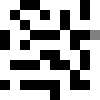
\includegraphics[scale=1.25]{images/maze_world_example.png}
\caption{Maze World Example: White spaces are open, Black spaces are blocked, and the Gray space is the goal.}
\label{fig:maze_world_example}
\end{figure}
As shown in the figure, the world is composed of 100x100 pixels but only represents a 10x10 maze.  These mazes were generated in python using example code from~\cite{maze_code} which creates an $m x n$ grided maze in an $M x N$ pixel image, where $m$ and $n$ are factors of $M$ and $N$ respectively.  At any white space in the maze there exists a path to any other white space on the maze that is unobstructed by a black space.  This allows the goal to be put at any open white space in the maze. To make the dataset simpler, the mazes were converted into a single-channel 8-bit integer representation.  

An agent is placed in the maze randomly in any white space.  The agent is represented by a smaller dark gray square as shown in Fig.~\ref{fig:maze_with_agent}. The goal of the agent is to make it to the goal in the least number of steps.  The agent has four possible actions; Move Right, Move Down, Move Left, Move Up. Actions are one-hot enconded. If the agent hits a wall (black) it loses, if it hits the goal it wins. At each step, the agent moves a full grid step.  In the back-end, the maze is treated like a $m x n$ grid, and Python's PIL framework is used to generate the graphics used for simulation and dataset generation.
\begin{figure}
\centering
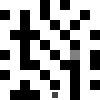
\includegraphics[scale=1.5]{images/maze_with_agent.jpg}
\caption{Maze World with Agent: small, dark gray square represents agent.}
\label{fig:maze_with_agent}
\end{figure}

\subsection{Expert Data}
Expert data is needed to teach an agent through demonstration.  To generate expert data, a maze is created and an agent is placed randomly inside of the maze at any valid space. Then using Python's networkx library the 2D grided maze is converted into a graph.  Then using the networkx function $single\_source\_shortest\_path()$ every path from a valid point to the goal is computed using Dijkstra's algorithm. These paths are then used to allow the agent to traverse through the maze to the goal in the least amount of steps possible.

\subsection{Random Data}
\label{sec:random_data}
Random data is needed to ensure that the agent is able to have experience at every space in the maze.  Expert data will be able to hit many of these spaces, but it will only ever choose one action (the optimal action) in these spaces. To generate random data, a maze is created and an agent is place randomly inside of the maze at any valid space.  The agent then takes any valid action randomly to move to another valid space, this action does not necessarily have to be optimal. This data does not continue after this, only the original state of the agent, the action taken, and state after action of the agent is stored.

\subsection{Datasets}
Expert data and random data are stored as GIFs.  To do this, at each movement of the agent an image is generated (such as in Fig.~\ref{fig:maze_with_agent}) to represent the current state of the agent in the maze.  For expert data these images are collected until the agent reaches the goal. The images are then combined into a GIF and saved for later use.  Each action the agent takes is saved into a text file to be used later. The same is done for the random data, except that the GIFs were only two images total.

Two types of datasets were created for expert data and random data; same and random.
\subsubsection{Same}
"Same" means that the maze the agent is in does not change.  Therefore, the expert data and random data use the same maze, however the placement of the agent will change.  This dataset is used to show whether or not a system can learn a single task without generalizing what the task is.

\subsubsection{Random}
"Random" means that the maze the agent is in does change.  Therefore, the expert data and random data use different randomly generated mazes, and the placement of the agent changes in each maze.  This dataset is used to show whether or not a system can learn a single task while also generalizing what the task is.

\subsection{Simulation}
Given a maze, current placement of the agent, and the action to be performed, a simulation of the maze task can be completed.  This is used in testing as well as in training to show how well the agent is learning and to gather data.  At each step the simulation environment tells the system the new state of the agent (image of maze with agent), whether or not the agent has reached the goal, and whether or not the agent has crashed into a wall.  If the simulation is fed an initial maze image, it will keep that maze for the rest of the simulation (in cases where the same maze is being tested) otherwise it will use a random generated maze.  If the simulation is given no initial state, it will randomly place the agent in the maze.

\subsection{Processing Data}
To make the saved GIFs and action-list text files usable to the system architectures, some preprocessing needs to be done.  First, the GIFs are read in frame by frame.  These frames are then converted to the data size needed using PIL image resize function.  These are then saved into a numpy array of shape $[?,data size, data size, 1]$.  As shown, all the data is square.  The actions are read out of the action-list and converted into one-hot encoded vectors stored into a numpy array of shape $[?,number of actions]$.  These arrays are then split into test, train, and reward datasets for the image data and action data.  These split arrays are then stored into an h5py file so that it can be accessed faster and more efficiently when the system is run again. 

%\chapter{Technologies and Implementations}
%\section{TensorFlow}

\chapter{Proposed Architectures}
\section{Deep Apprenticeship Learning (DAL) Architecture Modification}
\subsection{No Pooling Layers}
One issue with the Deep Apprenticeship Learning (DAL) architecture in~\ref{sec:DAL}, is its use of pooling layers.  Pooling does well in classification to increase performance, however it removes many fine details that are necessary in task completion and understanding.  Removing the pooling after each convolution layer results in slower training, but allows the network to learn from smaller details within the images given.  For example, the using Maze World, pooling layers would remove the goal and the agent from existing after the first layer, causing all of the states going through the network to look almost identical.  This was shown in testing the DAL network when it would predict the same action be taken for each state presented.
\subsection{Transfer Learning}
Another change to the DAL architecture is the use of transfer learning.  In the current implementation of DAL, the DAQN and DARN are trained seperatley.  This means that, while they use the same network architecture, the DARN network starts with random weights and biases to learn from the DAQN network.  Instead, using a methodology called transfer learning, the DARN network is initialized with the same weights as the DAQN network before being trained.  This allows the DARN network to have a good starting point in understanding the structure of the states so that its main focus is on updating its Q-values and not processing the image.  This also allows it to learn faster, and with a lower cost.
\subsection{Using Q-Learning}
On top of removing pooling layers and including transfer learning, methodologies from Q-learning were also implemented.  In its current form, the DAQN network in DAL does not use Q-updates to compute its loss.  Instead it uses the softmax of the output of the network to compare it to the action it is supposed to be.  While a method like this would work in classification, it is unstable in task learning because it leads to large jumps in updating the weights of the network.  Instead the loss function was changed to be more representative of Q-learning for both the DAQN and DARN networks as shown in~\ref{eq:dal-dqn-loss}

\begin{equation}
     \label{eq:dal-dqn-loss}
     \resizebox{0.5\textwidth}{!}{$J(Q) =(R(s,a)+\gamma*max_{a'}Q(s',a'))-Q(s,a))^2$} 
\end{equation}
\subsubsection{Reward Abstraction}
An inherit issue with this representation is the need for the reward $R$.  The purpose of apprenticeship learning is to find the reward model from given expert demonstrations, which means that the reward for each step an agent or expert takes is not known. By abstracting the reward function from step-level to task-level, it serves as a task completion modifier for the loss.  For example, for each step taken by the expert if the task is not complete the reward is $0$, if the task is complete the reward is $+1$, and if the task is failed the reward is $-1$.  Since the expert data used is all successful, only the last transition for the expert into the goal is given a reward of $+1$.  For the DARN network, the same loss function is used, but instead of using random data (\ref{sec:random_data}) the network "plays against itself" to accrue more experience.  Therefore, the agent starts in a maze in a random location and performs a step based on the network output from the state it is in.  If the step is to the goal the reward is $+1$ if it hits a wall it is $-1$ (and the maze resets), otherwise it is $0$.  

\subsubsection{Experience Replay}
Upon creating experiences using the DARN network, the network will be updated through min-batches of experiences in the form of $(s,a,s',r)$ once its replay buffer is full.  As the agent has more experiences the older experiences are overwritten by the newer ones.  This allows the network to learn only from the most recent experiences to weed out "bad habits" from earlier experiences. 

\section{Deep Q-Networks Implementations}
Many success have been seen in the realm of Deep Q-Learning and its modifications.  While this does extremely well in reinforcement learning, its methodologies have not been used much in deep apprenticeship learning.  Two methodologies from this space include shared experience and dueling deep Q-networks.  Both of these network modifications use the Deep Q-Network architecture~\cite{atari} which is fully convolutional, and has been proven successful in task completion environments in the Atari world.
\subsection{Using Shared Experience}
Experience replay~\cite{atari} has been shown to lead to better learning in networks by using past experience.  However, up until now, in traditional reinforcement learning only the agent's experience was used with this method.  While this worked for algorithms that relied on exploration and exploitation, it did not always produce great results if the experiences were not successful. This may cause the network to hit a local minima where the optimal action selection will never be reached. In apprenticeship learning, experiences from an expert are given and are guaranteed to be correct.  Using these experiences along with the agent's learned experiences would allow for better learning.  Hester et al.~\cite{hester2017learning} introduced this in their DQfD architecture, and showed that just using 10\% of expert data in each batch update of experiences gave way to better learning, and ensured that the agent was not going to keep relearning from bad experiences.  This also ensures that the network can get out of a local minima and continue learning despite the "bad" learned experiences.
\subsection{Target Q-Network}
Mnih et al.~\cite{atari} also introduced the concept of using a separate target Q-network.  This was due to the fact that the Q-network architecure is unstable along sequential updates.  By updating the weights of the Q-network by small amounts every iteration, the network is more likely to diverge due to tightly coupled correlations.  A target Q-network is used outside of the main Q network.  The main Q-network is updated at each iteration using values from the target Q-network.  After $\tau$ iterations, the target Q-network's weights are updated with main Q-network's weights. 
\subsection{Using Dueling DQN}
Another modification made was using the Dueling Deep Q-Network architecture (\ref{sec:DuelingDQN})~\cite{wang2015dueling}.  By splitting the value and advantage functions from the main Q-network, allows for the separation of state estimation and action selection.  By decoupling these two, the network can more accurately predict the best action to take regardless of the state that was predicted. For the dataset used (Maze World), this allows for part of the network to determine the current maze and placement of the goal, and the other part of the network to determine the shortest point to that goal. 

\chapter{Results}

Table of Task Completion (Same)~\ref{tab:task-complete}
\begin{table}[]
\centering
\caption{Task Completion Results}
\label{tab:task-complete}
\begin{tabular}{|l|l|l|}
\hline
\multicolumn{3}{|c|}{Task Completion Results} \\ \hline
\textit{\textbf{Networks}} & \textit{\textbf{Tests Completed}} & \textit{\textbf{Correct Action Prediction}} \\ \hline
DAL &  &  \\ \hline
DAL with Transfer Learning (no pooling) &  &  \\ \hline
DAL with Bayesian Implementation &  &  \\ \hline
DQN-AL & 2/10 & 18.4\% (23/125) \\ \hline
Dueling DQN-AL & 9/10 & 76.8\% (96/125) \\ \hline
\end{tabular}
\end{table}

Table of Task Understanding (Random)~\ref{tab:task-understanding}
\begin{table}[]
\centering
\caption{Task Understanding Results}
\label{tab:task-understanding}
\begin{tabular}{|l|l|l|}
\hline
\multicolumn{3}{|c|}{Task Understanding Results} \\ \hline
\textit{\textbf{Networks}} & \textit{\textbf{Tests Completed}} & \textit{\textbf{Correct Action Prediction}} \\ \hline
DAL &  &  \\ \hline
DAL with Transfer Learning (no pooling) & 2/10 & 11.6\% (11/95) \\ \hline
DAL with Bayesian Implementation &  &  \\ \hline
DQN-AL & 0/10 & 9.5\% (9/95) \\ \hline
Dueling DQN-AL & 1/10 & 13.7\% (13/95) \\ \hline
\end{tabular}
\end{table}

Include loss graphs

Include example images in sequence

Table of results

\chapter{Conclusions and Future Work}


Future Work
- Task specific, for maze have two networks one for agent location one for maze detection?


  \nocite{*}
%%%%%%%%%%%%%%%%%%%%%%%%%%%%%%%%%%%%%%%%%%%%%%%%%%%%%%%%%%%%%%%%%%%%%%%%%%%%%%%

%%%%%%%%%%%%%%%%%%%%%%%%%%%%%%%%%%%%%%%%%%%%%%%%%%%%%%%%%%%%%%%%%%%%%%%%%%%%%%%
\bibliographystyle{plain}
% Single space the bibliography to save space.
\begin{singlespace}
\bibliography{Thesis}
\end{singlespace}
%%%%%%%%%%%%%%%%%%%%%%%%%%%%%%%%%%%%%%%%%%%%%%%%%%%%%%%%%%%%%%%%%%%%%%%%%%%%%%%

%%%%%%%%%%%%%%%%%%%%%%%%%%%%%%%%%%%%%%%%%%%%%%%%%%%%%%%%%%%%%%%%%%%%%%%%%%%%%%%
% The appendices are (of course) optional.
\appendix
%\chapter{A Long Proof}
  ...
%%%%%%%%%%%%%%%%%%%%%%%%%%%%%%%%%%%%%%%%%%%%%%%%%%%%%%%%%%%%%%%%%%%%%%%%%%%%%%%
\end{document}